



Tal y como se menciona en el Capítulo 2, el objetivo principal de este proyecto radica en el desarrollo de un prototipo tal que ayude, permita y facilite el monitoreo alimenticio de un conjunto de novillos estabulados en proceso de engorde. Para ello primero es necesario comprender las etapas que influyen en la adquisición de datos y posteriormente considerar \textit{Oportunidades de Intervención} (\textit{OI}) o mejora desde un punto de vista ingenieril.\\

\section{Iteración diaria del proceso de engorde}

El proceso inicia con la verificación de alimento suficiente para el o los grupos de bovinos a alimentar, seguido por la entrada de individuos al área de alimentación; los animales deben ser ingresados por grupos de tal forma que se tenga conocimiento de los individuos que ingresan y salen, y de las porciones correspondientes para que su evolución y monitoreo alimenticio sea apropiado.

\begin{enumerate}[O.I \#1:]
    \item Esto sugiere la necesidad de identificar a los novillos y tener a la mano sus porciones dietarias correspondientes. \label{OI1}
\end{enumerate}

Al tener identificado al individuo y por ende tener conocimiento de su porción dietaria correspondiente, es necesario entregar dichas porciones descartando cualquier tipo de aproximación errónea, discrepancia o por ambigüedad por el criterio humano. Por otra parte se requiere optimizar el tiempo, costo y personal requerido en la dosificación del alimento desde el tanque de almacenamiento hasta los comederos.

\begin{enumerate}[O.I \#2:]
    \item Para validar y verificar que las porciones son apropiadas y  verídicas, se opta por pesar las porciones con balanzas digitales antes de ser entregadas al animal. En lo que respecta al suministro constante de alimento se considera tener puntos fijos de dosificación continua que faciliten la distribución del alimento de manera automática. Para ello se requiere la inclusión de mecanismos de dosificación como los mencionados en la Sección \ref{dosificadores}. \label{OI2}
\end{enumerate}

\begin{inparaenum}[(i)]
	        Una vez iniciada y finalizada la ingesta del alimento, el animal es llevado a una balanza para obtener su peso actual, seguido a esto se registra manualmente éste y otros datos concernientes a su proceso de alimentación tales como:
	        \item Las veces que ha sido alimentado
	        \item Si ha presentado alguna dificultad en consumir su ración diaria. Posteriormente se da salida del área de alimentación.
	    \end{inparaenum}

\begin{enumerate}[O.I \#3:]
    \item Al identificar al individuo mediante una referencia única, se pueden asociar datos a esta referencia de identificación, tal y como se realiza en una institución educativa mediante el carné estudiantil. Con esto, el registro de datos se garantiza de forma tal que no se puedan asignar datos erróneos entre los novillos del ganado estabulado ocurridos por equivocaciones en el registro manual de datos. 
    Además, si el peso ha presentado algún comportamiento deseable o indeseable, el registro estadístico de los datos puede aportar en la toma de decisiones futuras. \label{OI3}
\end{enumerate}

Finalmente y de forma iterativa, se debe verificar que haya alimento suficiente para un próximo grupo que ingrese al área de alimentación.\\

Como ayuda gráfica para abstraer el sistema, se considera el siguiente diagrama de actividades general mostrado en la Figura \ref{dblockspng}:

\begin{figure}[H]
	\begin{center}
		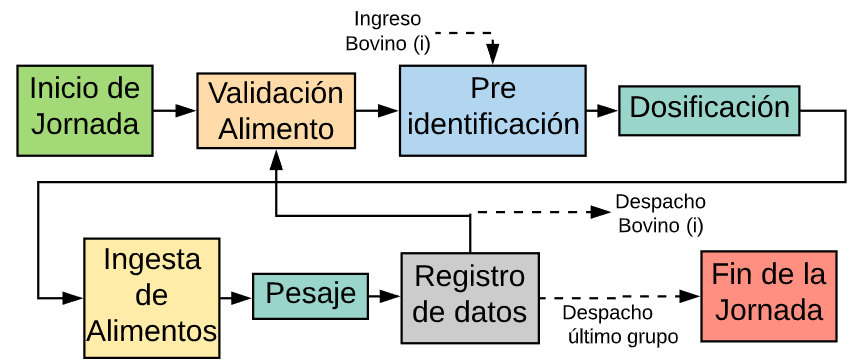
\includegraphics[scale=0.85]{img/dblocksg.png}
	\end{center}
	\caption{Diagrama de actividades general. \label{dblockspng}}
\end{figure}

Del diagrama se puede describir lo siguiente:

\begin{itemize}
	\item Para la verificación y validación del alimento se pueden utilizar sensores de presencia que indiquen la existencia (o no) de alimento suficiente.
	\item Para la ``Pre-identificación'', se puede hacer uso de los dispositivos RFID mencionados en la sección \ref{concepadic} y atendiendo a la OI \#\ref{OI1}. %%% Tek -> Observación Resuelta
	\item Para la ``Dosificación'' del alimento se requiere de hardware, sensores y actuadores electrónicos y/o electromecánicos.
	\item Para el registro de los datos se puede hacer uso de la etapa de ``Pre-identificación'' y asociar bases de datos a estos dispositivos de reconocimiento para que se actualicen los datos de manera inequívoca.
% 	\item C.I. hace referencia a las condiciones iniciales necesarias para ejecutar las actividades.
\end{itemize}

Con base en lo anterior, se puede relacionar la iteración diaria del proceso de engorde mediante un sistema prototipo segmentado en 4 subsistemas principales  que son descritos a continuación:

\begin{itemize}
    \item ``Identificación'': Subsistema para la identificación del ganado.
    \item ``Estructura mecánica'': Composición física y mecánica del sistema prototipo.
    \item ``Hardware'': Medición de variables de interés y manejo de actuadores.
    \item ``Procesamiento de datos'': Tratamiento de los datos obtenidos.
\end{itemize}

% Observación añadida Post Sustentación el día 29 DE Julio de 2020 por comentarios del Jurado Carlos Lozano
\textit{\textbf{Anotación complementaria: }} En secciones posteriores se muestran análisis y selección de alternativas para cada uno de los subsistemas (si aplica), mediante el uso de matrices de selección como las Tablas \ref{matrizid}, \ref{matrizactpng} y \ref{matrizmotor}. Los valores enteros de los pesos (1 a 5) y la ponderación de los valores allí registrados dependen de las siguientes consideraciones:

\begin{itemize}
    \item Criterio personal: Algunas alternativas requieren de experiencia en el manejo de otras ciencias aplicadas como la mecánica o la agropecuaria, por lo que dado el caso, los pesos asignados para la Tabla \ref{matrizactpng} dependerán de las capacidades, herramientas, recursos económicos, recursos humanos y criterios propios del estudiante autor de este proyecto de grado.
    \item Criterio comercial: Las alternativas planteadas están sujetas a costos que pueden ser altos o bajos por lo que se considera de manera personal la capacidad económica del estudiante para la selección de una alternativa sobre otra.
    \item Criterio económico: Las alternativas están sujetas a precios variables según su funcionalidad, calidad y cantidad. Estos gastos serán suplidos acorde a las capacidades económicas del estudiante, por lo tanto es éste quien puede escoger las alternativas que mejor se acomoden a su presupuesto.
    \item Consideraciones convencionales: Algunas alternativas pueden poseer características que las hagan aparentemente más útiles que otras, no obstante se busca una simplificación de elementos comerciales, electrónicos y mecánicos, por lo que para la Tabla \ref{matrizmotorpng}, la asignación de los pesos se ve influenciada por la simplicidad de mantenimiento y uso de una alternativa sobre otra.
    \item Criterios comparativos: Las alternativas están sujetas a comparaciones entre las mismas, se tiene en cuenta su complejidad, sus características y su implementación por parte del autor del proyecto.
    \item Alternativas que se alejan de dichas condiciones serán atribuidas con pesos bajos (1) y aquellas que se acerquen o mejoren dichas condiciones serán atribuidas de pesos altos (5).
\end{itemize}

Con base en lo anterior, un valor de 1 será asignado para alternativas que se consideren como poco viables, malas, o no apropiadas. De manera análoga, un valor de 5 será asignado para alternativas que sean consideradas apropiadas. Todo esto con respecto a estos y demás criterios de selección mencionados más adelante.

% \pagebreak

\section{Subsistema de Identificación (ID)}\label{subsisid}
%	\item \textbf{ID: } 
%	El dispositivo RFID es asignado a cada novillo de engorde, y éste lo portará . /*ESTO LO PONGO EN EL QUE YO ESCOGÍ*/
	En el subsistema de Identificación se realiza la identificación de cada novillo mediante un accesorio, característica, marca, descripción, nombre o finalidad. Sin embargo, por cuestiones de recursos, facilidad de uso, utilidad descriptiva e informativa y capacidad de reutilización, se requiere seleccionar una modalidad de las mencionadas en la sección \ref{identiganado}, que cumpla parcial o totalmente con estos criterios.\\
	
	Para seleccionar la alternativa más apropiada se procede a realizar una matriz de selección de peso ponderado bajo los siguientes dictámenes:
	
	\begin{itemize}
	   \item Los pesos asignados para cada criterio son valores enteros del 1 al 5.
	   \item Entre mayor sea el peso asignado, significa que la modalidad es más apropiada para cada criterio de selección.
	   \item \begin{inparaenum}[(i)]
	        Los criterios usados para esta matriz son:
	        \item ``Costo''
	        \item ``Reutilizable''
	        \item ``Manipulable''
	        \item ``Informativo''
	    \end{inparaenum}
	    \item El criterio de costo representa la relación costo beneficio que representa cada alternativa.
	    \item El criterio reutilizable representa la posibilidad de reciclar su uso para futuras ocasiones y que no sea desechable o de único uso.
	    \item El criterio manipulable hace referencia a qué tan intuitivo es y  qué tan fácil es de manejar por terceros.
	    \item En cuanto al criterio Informativo, como su nombre lo indica, éste representa cuán descriptivo e informativo es en cuanto a una res en específico, ya sea por edad, género, raza, todas las anteriores o ninguna.\\
	    
	\end{itemize}
	
	Con base en lo anterior se obtiene la siguiente matriz de pesos:
\begin{table}[H]
\centering
\caption{Matriz de selección por peso ponderado para el subsistema ID. \label{matrizid}}
\begin{tabular}{|c|c|c|c|c|c|}
\hline
\multirow{3}{*}{Alternativas} & \multicolumn{4}{c|}{Criterios} & \multirow{3}{*}{\begin{tabular}[c]{@{}c@{}}Valoración final\\   de la alternativa\end{tabular}} \\ \cline{2-5}
 & 30\% & 25\% & 15\% & 30\% &  \\ \cline{2-5}
 & Costo & Reutilizable & Manipulable & Informativo &  \\ \hline
Arete & 4 & 1 & 4 & 3 & 2,95 \\ \hline
Chip Subcutáneo & 3 & 1 & 4 & 5 & 3,25 \\ \hline
Jáquima / Collar & 5 & 4 & 3 & 1 & 3,25 \\ \hline
Marcado & 4 & 1 & 2 & 2 & 2,35 \\ \hline
Nariguera & 4 & 3 & 2 & 1 & 2,55 \\ \hline
% Jáquima RFID & 5 & 4 & 4 & 5 & 4,6 \\ \hline
\end{tabular}
\end{table}	
% \begin{figure}[H]
% 	\begin{center}
% 		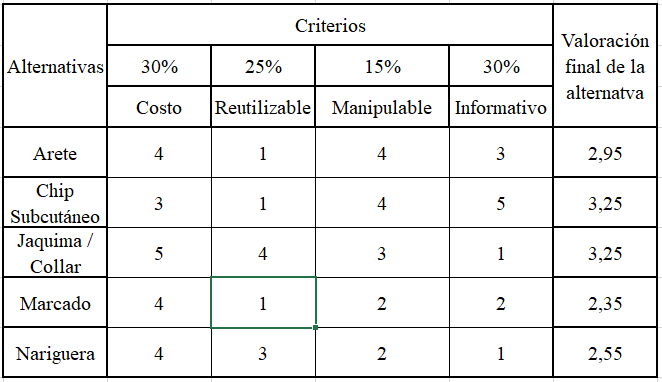
\includegraphics[scale=0.85]{img/matrizid.png}
% 	\end{center}
% 	\caption{Matriz de selección por peso ponderado para el subsistema ID. \label{matrizidpng}}
% \end{figure}


	       % 
	       % 

% De esta forma:}
% \begin{itemize}
%     \item  Respecto al criterio de ``Costo'', un valor de 1 significa que el precio es demasiado elevado ($\frac{\+\$30.000}{Uso}$, aproximadamente) y 5 significa que el precio es económico ($\frac{\-\$10.000}{Uso}$, aproximadamente) para los beneficios que ofrece la alternativa.
%     \item  Respecto al criterio ``Reutilizable'', un valor de 1 significa que la alternativa es desechable mientras que un valor cercano a 5 demuestra que la alternativa puede reutilizarse a futuro ($\frac{\5 Usos}{Unidad}$).
%     \item Respecto al criterio ``Manipulable'', Un valor de 1 significa que la alternativa es difícil de utilizar por terceros mientras que un valor cercano a 5 significa que es intuitiva y amigable para los usuarios (productores o personal ganadero).
%     \item Respecto al criterio ``Informativo'',Un valor cercano a 1 quiere decir que la alternativa puede entregar información subjetiva o ambigua, mientras que un valor cercano a 5 significa que se puede obtener atributos y descripciones pertinentes a una res de ganado de manera eficiente.
% \end{itemize}
	

	
	
	
De esta tabla se puede observar que de las 5 modalidades actuales más utilizadas en la ganadería (ver sección \ref{identiganado}), prevalece el uso de la jáquima o collar y el uso de un chip subcutáneo RFID.
Desde un punto de vista de la ingeniería electrónica, la modalidad que optimiza la identificación del ganado en cuestión de tiempo y facilidad de descripción informativa es la identificación mediante el transponedor de radiofrecuencia. Por otro lado, desde un punto de vista financiero, el uso del chip subcutáneo significa un elevado costo en comparación al uso de Collares que además de ser económicos  pueden ser reutilizables.

No obstante, aunque ambas opciones han resultado ser convenientes, se opta por buscar alternativas que permitan aprovechar los mejores atributos de ambas modalidades. Como resultado se opta por combinar estos atributos en una alternativa híbrida (Jáquima RFID) cuyo análisis y diseño se describe a continuación:

\subsection{Análisis}
 Para esta alternativa híbrida se requiere de 2 partes principales: el punto de lectura RFID, y el accesorio ``RFID tag''. Antes de proponer un primer diseño se opta por observar las condiciones de infraestructura convencional en este tipo de ganado estabulado para disponer de los puntos de lectura y por lo tanto la ubicación física del tag.
  
  \begin{figure}[H]
		\begin{center}
			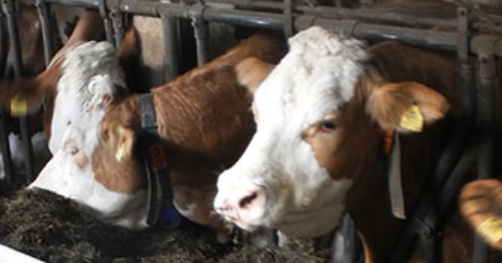
\includegraphics[scale=0.75]{img/barras.png}
		\end{center}
		\caption{Separación de ganado en el comedero.  Tomada de \cite{googlepics}. \label{barraspng}}
	\end{figure}
  
 Como se puede observar en la Figura \ref{barraspng}, el ganado estabulado se encuentra separado entre sí mediante puestos individuales de alimentación a los que son ingresados. Además, accede a su alimento al pasar su cabeza y cuello a través de un arreglo de barras que bordean la nuca; este arreglo varía de forma y tamaño acorde al tipo de res y se utiliza para evitar disputas en la manada.\\
 \begin{inparaenum}[(i)]
	        Con base en lo anterior se puede establecer que el lector RFID deberá estar posicionado en:
	        \item  Dentro o fuera del puesto de alimentación individual.
	        \item  En algún punto del arreglo de varillas que bordea la nuca del animal.
 \end{inparaenum}
 
 
\subsection{Diseños}
% \begin{itemize}
	\subsubsection{Diseño 1, Arnés, Chaleco ó ``Backband''}
	En primera instancia se considera un chaleco usable, portable y reutilizable, que sería utilizado por cada individuo perteneciente al ganado estabulado desde su ingreso hasta su salida en la etapa de ceba; es decir, hasta que alcance un peso adecuado para ser transformado en carne para consumo humano y una vez esto ocurriera, el chaleco sería reasignado a un próximo nuevo miembro de la etapa de engorde.
		
	Como los equinos, bovinos y otros animales domésticos ya utilizan accesorios en su día a día, se consideró posible que el ganado usase este tipo de complemento. Por otra parte, uno de los objetivos principales de este proyecto es que se pueda identificar cada una de las reses de manera automática y eficiente, por lo que el uso de etiquetas RFID (ver Figura \ref{rfidtagpng}) fue uno de los influyentes más importantes en este diseño.
	
	\begin{figure}[H]
	\begin{center}
		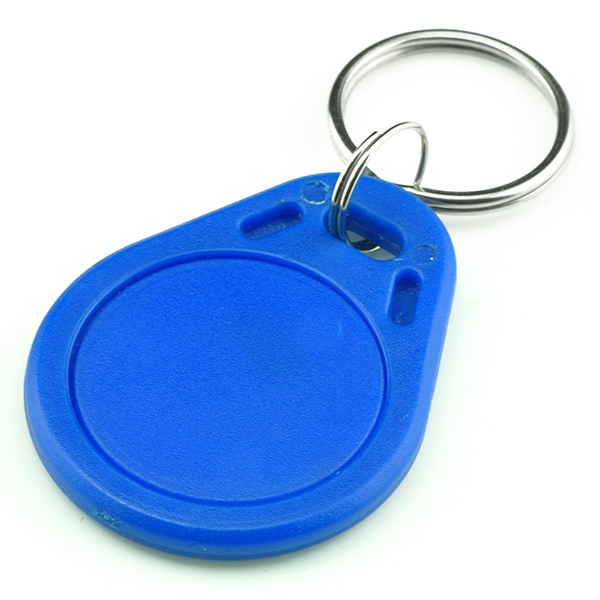
\includegraphics[scale=0.25]{img/rfidtag.png}
	\end{center}
	\caption{Etiqueta ó ``Tag'' RFID. Tomada de \cite{googlepics}. \label{rfidtagpng}}
	\end{figure}

% Ahora bien, en la infraestructura general de un comedero para ganado estabulado, se tienen algunas observaciones que por lo general son añadidas a la misma, como por ejemplo, la separación de cada cabeza mediante barras a los costados que sirven para separar a los animales entre sí evitando disputas en la manada (Ver Figura \ref{barraspng}).
%   Estas barras también rodean la nuca del animal dejando un espacio apropiado para que éste pueda ingresar su cabeza y cuello hasta el comedero.
% de canoa, canaleta o mixto.

% 		\begin{figure}[H]
% 		\begin{center}
% 			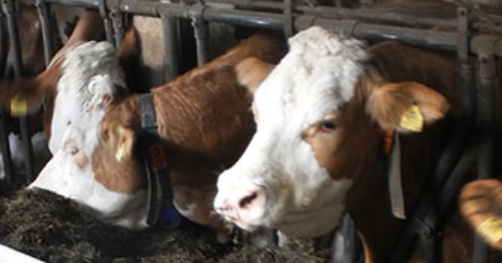
\includegraphics[scale=0.55]{img/barras.png}
% 		\end{center}
% 		\caption{Separación de ganado en el comedero. \label{barraspng}}
% 		\end{figure}
		
Además, para no requerir de un encargado de la lectura de cada ``RFID tag'' en los chalecos, es necesario que el lector se encuentre en una posición fija. Con esto en mente, se presupuso que el lector debería estar en un punto estratégico que facilitara la proximidad de la etiqueta RFID sin incomodar al individuo que sería alimentado.\\

Por lo tanto, el lector RFID se encontraría en la barra superior que bordea la nuca del bovino y por consiguiente la etiqueta RFID del chaleco se encontraría cerca de la ultima vértebra cervical.

Se diseñó un primer bosquejo en 3D del chaleco que contendría la etiqueta RFID y de la cual se colocarían las correas ajustables que bordearían el cuerpo del novillo (Ver Figura \ref{mod1png}),  

		\begin{figure}[H]
		\begin{center}
			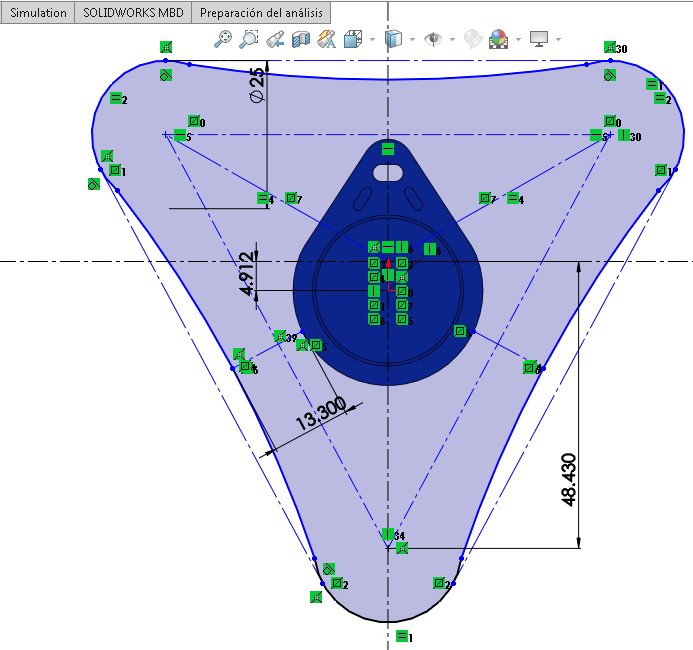
\includegraphics[scale=0.45]{img/primermodel.png}
		\end{center}
		\caption{Primer modelo 3D del compartimento RFID. \label{mod1png}}
		\end{figure}

Lastimosamente se detectó una primer falencia a este diseño, esto debido a que no todas las razas de bovinos más usados en este tipo de ganadería en Colombia son iguales en altura, contextura y fisionomía \cite{razas}. En la Figura \ref{jorobapng} se puede observar razas como la Cyr, Brahman y Nelore; estas poseen una especie de joroba en la nuca o tejido descolgado en la parte inferior del cuerpo, lo que complica el uso de los chalecos y de la posición de la etiqueta RFID en ellos.

		\begin{figure}[H]
		\begin{center}
			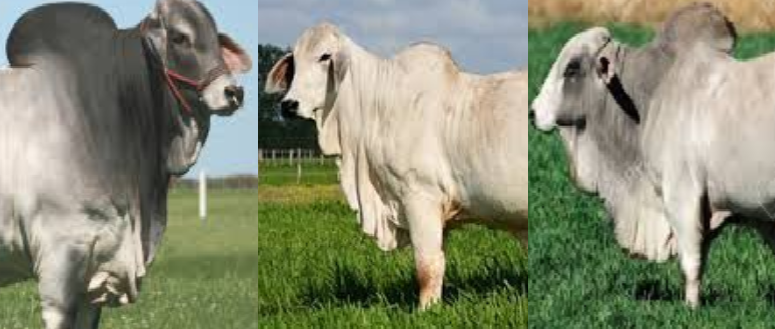
\includegraphics[scale=0.7]{img/joroba.png}
		\end{center}
		\caption{Fisionomía de razas comunes en el ciclo productivo de la Carne. Tomada de \cite{fisio1}. \label{jorobapng}}
		\end{figure}

\subsubsection{Diseño 2, ``Armband''}
Como medida reactiva o correctiva al problema del diseño anterior, se consideró que la etiqueta RFID podría ubicarse a uno de los costados de las extremidades del individuo y por ende el lector tendría una nueva ubicación acorde a este cambio. No obstante se presentaron otras complicaciones que evidenciaron fallas en este diseño.

La abrazadera ubicada en la extremidad, dificulta el movimiento articular de la misma y como en cualquier otro caso de interacción animal que vive en grupo, se presentan ocasiones de confrontación física entre sujetos del sexo masculino; estas confrontaciones pueden suponer un daño irreparable en el compartimento portable del ``Armband'' dificultando la identificación del bovino en ocasiones futuras.\\
		
% 	\end{itemize}
		
\textit{\textbf{Anotación:} Para conservar factores característicos como la portabilidad, usabilidad, reutilización del identificador RFID y recalcando lo aprendido sobre las falencias de los diseños anteriores, se decide combinar el uso de la Jáquima y los 2 prototipos diseñados con la etiqueta RFID dando como resultado el siguiente diseño:}

\subsubsection{Diseño 3, ``Jáquima RFID''}
 
Para el diseño de este nuevo prototipo se observa que un rasgo físico común entre las razas de bovinos usadas para engorde, es  que poseen un gran espacio en la parte frontal del cráneo, por encima de los ojos y que suelen usarse jáquimas comerciales, convencionales, modificables, etc.\\

En la figura \ref{argollapng} se observa que las Jáquimas especializadas utilizan una argolla de conexión para unir y tensionar las correas ajustables. Teniendo esto presente, se puede reemplazar o adaptar un accesorio que se acople a las correas y que pueda portar una etiqueta RFID.

		\begin{figure}[H]
		\begin{center}
			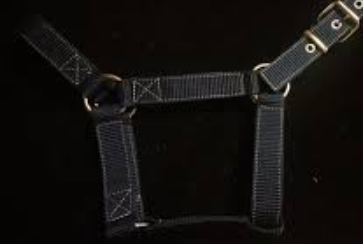
\includegraphics[scale=0.9]{img/argolla.png}
		\end{center}
		\caption{Argolla de conexión. \label{argollapng}}
		\end{figure}

Nuevamente, el diseño 3D de este accesorio se realiza en SolidWorks. En este caso, el diseño requiere de 2 partes. Primeramente se diseña la base, a la que se le condiciona un corte interno que sirve como almohadilla en donde se inserta la etiqueta RFID y también cuenta con 3 hendiduras para el acople de la tapa protectora.

        \begin{figure}[H]
		\begin{center}
			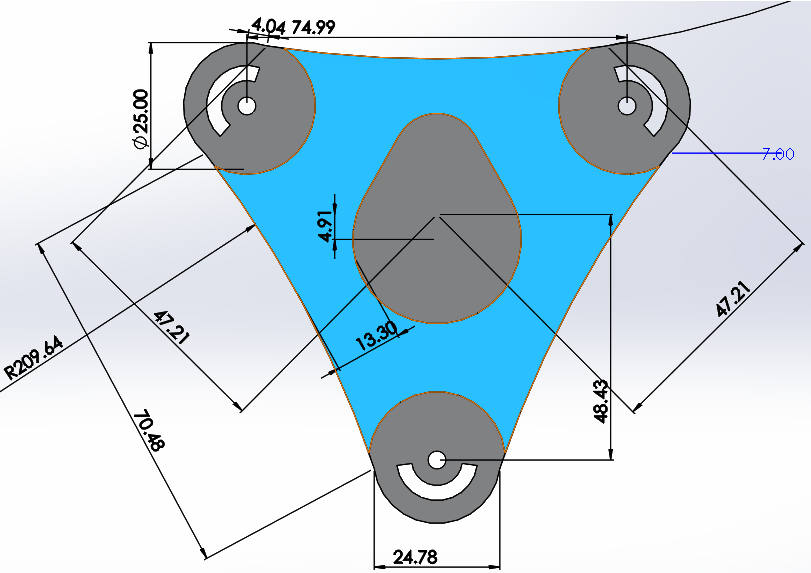
\includegraphics[scale=0.635]{img/medidasbase.png}
		\end{center}
		\caption{Medidas para la Base. \label{medidasbasepng}}
		\end{figure}

Así mismo la tapa protectora cuenta con 3 salientes que sirven para acoplarse correctamente a la base y permitir que se conforme el accesorio en su totalidad. En  el lado derecho de la Figura \ref{tapabasepng} se observa la primera parte usada como base y del lado izquierdo, la otra parte que servirá de tapa protectora.

        \begin{figure}[H]
		\begin{center}
			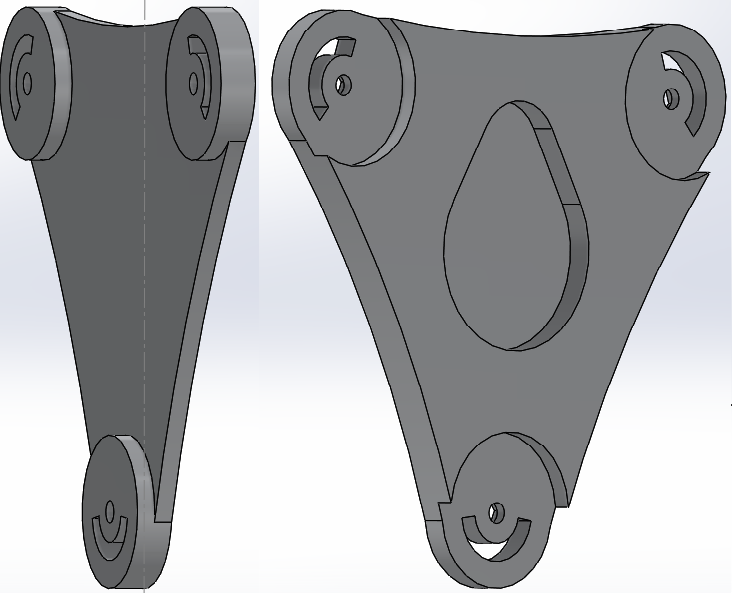
\includegraphics[scale=0.55]{img/tapabase.png}
		\end{center}
		\caption{Tapa y Base del accesorio para la Jáquima RFID. \label{tapabasepng}}
		\end{figure}

Es importante añadir que este accesorio permite cambiar la etiqueta RFID si lo requiere, lo que evidencia la reutilización del prototipo para ganado en el futuro.\\

Finalmente, al ensamblar la base y la tapa del accesorio junto con unas abrazaderas ajustables, se finiquita el accesorio prototipo denominado como ``Jáquima RFID''. Este contiene un identificador único (UID) que se encuentra grabado en la memoria de la etiqueta RFID añadida al mismo.
%   para la identificación del ganado estabulado:

\begin{figure}[H]
	\begin{center}
		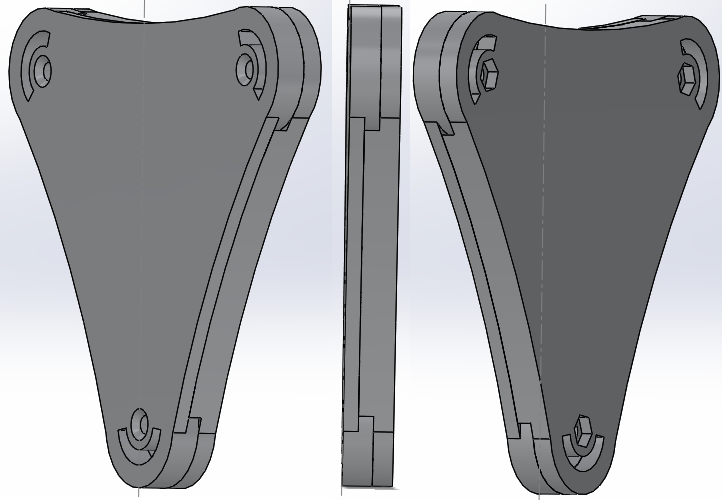
\includegraphics[scale=0.55]{img/jaquimaidsimul.png}
	\end{center}
	\caption{Jáquima ID. \label{jaquimaidpng}}
\end{figure}

% \end{itemize}

 Por su parte para este último diseño se requiere que el lector del dispositivo RFID deba posicionarse en un lugar que esté en contacto con la parte frontal del novillo. Siguiendo este orden de ideas y teniendo en cuenta que se presentarán distintos ejemplares de diferentes tamaños y fisonomías; el punto estratégico de lectura sería la puerta de ingreso al puesto de comida. Además, como los animales son guiados a estos puestos con la ayuda de personal calificado, el registro en la entrada es el punto más apropiado para garantizar que el individuo ingresado está (o no) identificado para su alimentación y estudio correspondiente.
Así pues, se concluyen los diseños de este subsistema satisfaciendo la O.I \#\ref{OI1} y el objetivo especifico #4 donde los novillos que cuenten con este accesorio podrán ser debidamente identificados a la hora de ser ingresados a los puestos de comida donde se les dosifica el alimento.
\pagebreak
% Con base en lo anterior se incluye este diseño como alternativa dentro de la tabla \ref{matrizid} obteniéndose un peso ponderado superior debido a que se logran aprovechar las mejores características posibles.

% \begin{table}[H]
% \centering
% \begin{tabular}{|c|c|c|c|c|c|}
% \hline
% \multirow{3}{*}{Alternativas} & \multicolumn{4}{c|}{Criterios} & \multirow{3}{*}{\begin{tabular}[c]{@{}c@{}}Valoración final\\   de la alternativa\end{tabular}} \\ \cline{2-5}
%  & 30\% & 25\% & 15\% & 30\% &  \\ \cline{2-5}
%  & Costo & Reutilizable & Manipulable & Informativo &  \\ \hline
% Arete & 4 & 1 & 4 & 3 & 2,95 \\ \hline
% Chip Subcutáneo & 3 & 1 & 4 & 5 & 3,25 \\ \hline
% Jáquima / Collar & 5 & 4 & 3 & 1 & 3,25 \\ \hline
% Marcado & 4 & 1 & 2 & 2 & 2,35 \\ \hline
% Nariguera & 4 & 3 & 2 & 1 & 2,55 \\ \hline
% Jáquima RFID & 5 & 4 & 4 & 5 & 4,6 \\ \hline
% \end{tabular}
% \caption{Matriz de selección por peso ponderado para el subsistema ID final. \label{matrizidfinal}}
% \end{table}	

\pagebreak
\section{Subsistema  de Estructura Mecánica} \label{subsishw}

	El subsistema Mecánico comprende la estructura tangible (estante, carcasa, armadura), en donde se realiza la activación de los dispositivos electrónicos (Hardware) y mecánicos encargados de validar y dosificar el alimento desde el tanque de almacenamiento hasta el ``plato'' de comida del novillo (comedero). Este subsistema está divido en 3 partes principales: La primera parte consta de la conexión física y mecánica de las partes que comprenden el punto de dosificación (tolva, mecanismo de dosificación, accesorios de conexión, etc). La segunda parte abarca el funcionamiento en conjunto del mecanismo de dosificación para extraer el alimento desde la tolva hasta un punto de validación de pesaje. Por último, se tiene una etapa de conexión entre el pesaje de la porción y el punto de alimentación del bovino.
	
\subsection{Análisis}
\subsubsection{Tanque de almacenamiento}
    
    De acuerdo con lo mencionado al inicio de la sección \ref{dosificadores} y retomando la estructura general de un dosificador como el de la Figura \ref{dosif2png}, es considerable que el sistema prototipo cuente con una estructura física similar. No obstante en la ganadería convencional, el alimento almacenado suele encontrarse en tanques, zonas o cuartos aislados, lejos del alcance de los animales y por lo tanto del establo de alimentación. Día a día se transportan desde estas zonas hasta los establos de alimentación, las cantidades de alimento requeridas para abastecer el ganado. Sin embargo, esto retarda la jornada diaria del proceso de ceba para grandes poblaciones de ganado.
	
	\begin{figure}[H]
		\begin{center}
			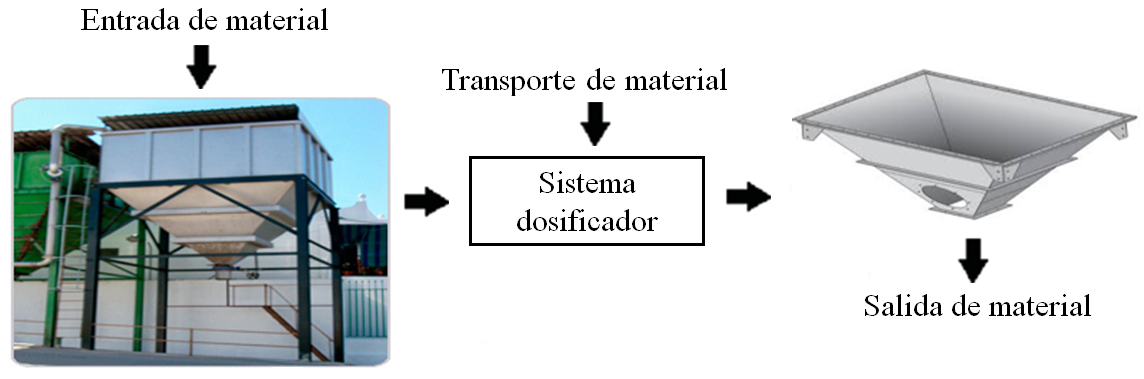
\includegraphics[scale=0.55]{img/dosificacion.png}
		\end{center}
		\caption{Estructura general de un dosificador. \label{dosif2png}}
    \end{figure}
	
	Con base en lo anterior, se plantea almacenar el alimento dietario en tanques de menor tamaño (en comparación a una habitación de almacenaje) ubicados en los establos de alimentación. De esta manera el alimento dietario puede ser re-abastecido y suministrado en un mismo lugar. Así pues, la tolva del sistema dosificador sería a su vez el tanque de almacenamiento que estaría conectado con el sistema dosificador descrito más adelante.

\subsubsection{Mecanismo de dosificación}

    Está claro que existen diferentes mecanismos usados para manipular alimentos tanto de consumo humano como animal. Estos mecanismos poseen atributos, diseños y sistemas de funcionamiento con características especializadas para su propósito; estos varían dependiendo del tipo de alimento, la cantidad de alimento, precisión, velocidad de trabajo, entre otros criterios. 
    
	Para saber cuál de estos mecanismos se acomoda a las necesidades, limitantes, situaciones y propiedades del entorno de trabajo de este proyecto, nuevamente es necesario la selección de el(los) mecanismo(s) más apropiado(s). Para ello se recurre a realizar una nueva matriz de selección con los siguientes dictámenes:
	
	\begin{itemize}
	   \item Los pesos asignados para cada criterio son valores enteros del 1 al 5.
	   \item Entre mayor sea el peso asignado, significa que la modalidad es más apropiada para cada criterio de selección.
	   \item \begin{inparaenum}[(i)]
	        Los criterios usados para esta matriz son:
	        \item ``Costo''
	        \item ``Viabilidad técnica''
	        \item ``Manipulación electrónica''
	        \item ``Precisión de Dosificación''
	        \item ``Propósito adecuado''
	    \end{inparaenum}
	    \item El criterio de costo representa la relación costo beneficio que representa cada alternativa.
	    \item El criterio de viabilidad técnica representa la posibilidad de implementación factible y apropiada para la aplicación para la cual ha sido diseñada.
	    \item El criterio de manipulación electrónica hace referencia a qué tan complejo es su uso mediante intervención electrónica. 
	    \item En cuanto al criterio de precisión, representa cuán precisa es la alternativa para la dosificación de porciones establecidas.
	    \\
    \end{itemize}

\begin{table}[H]
\centering
\caption{Matriz de selección por peso ponderado para el mecanismo dosificador. \label{matrizactpng}}
\begin{tabular}{|c|c|c|c|c|c|c|}
\hline
\multirow{3}{*}{Alternativas} & \multicolumn{5}{c|}{Criterios} & \multirow{3}{*}{\begin{tabular}[c]{@{}c@{}}Valoración \\ final de la\\  alternativa\end{tabular}} \\ \cline{2-6}
 & 25\% & 15\% & 20\% & 15\% & 25\% &  \\ \cline{2-6}
 & Costo & \begin{tabular}[c]{@{}c@{}}Viabilidad\\   técnica\end{tabular} & \begin{tabular}[c]{@{}c@{}}Manipulación\\   electrónica\end{tabular} & \begin{tabular}[c]{@{}c@{}}Precisión de\\  dosificación\end{tabular} & \begin{tabular}[c]{@{}c@{}}Propósito  adecuado\\  (manejo de alimento)\end{tabular} &  \\ \hline
\begin{tabular}[c]{@{}c@{}}Compuerta \\ deslizante\end{tabular} & 3 & 3 & 2 & 2 & 4 & 2,9 \\ \hline
\begin{tabular}[c]{@{}c@{}}Compuerta \\ rotativa\end{tabular} & 4 & 4 & 3 & 2 & 5 & 3,75 \\ \hline
\begin{tabular}[c]{@{}c@{}}Tornillo \\ sin fin\end{tabular} & 3 & 4 & 4 & 5 & 4 & 3,9 \\ \hline
\end{tabular}
\end{table}


	Teóricamente, tanto el tornillo sin fin como la compuerta rotativa poseen propósitos de dosificación de alimentos,  viabilidad técnica similar y una buena relación costo-beneficio. El factor determinante en la selección de la alternativa más apropiada es la precisión de dosificación, en la que el tornillo sin fin supera  a la compuerta rotativa. Un criterio extra en el análisis es la lejanía entre los animales y el tanque de almacenamiento. Tal y como se pudo observar en la Figura \ref{dosifpng}, el alimento se encuentra en un tanque de almacenamiento y es transportado una cierta distancia hasta el punto de alimentación del animal.
	
	Entre mayor sea esta distancia de separación, menor es el riesgo que los animales puedan llegar a tener contacto directo con el tanque. Así pues,  el mecanismo encargado de extraer el alimento será el denominado ``Tornillo sin fin''.
	Como este mecanismo es en principio mecánico, su accionamiento debe ser controlado por una señal de activación por pulsos (PWM) ocasionada por señales provenientes del subsistema ID. Por otra parte, el tornillo debe moverse rotativa y constantemente gracias a un actuador electrónico como por ejemplo un motor. \\
	
	Una vez más, es imperativo seleccionar el tipo de motor más adecuado para culminar esta tarea. Por lo que en esta ocasión los criterios decisivos serán el costo, la manipulación electrónica, el torque del motor y el consumo energético.\\
	
\begin{table}[H]
\centering
\caption{Matriz de selección por peso ponderado para el motor.} \label{matrizmotor}
\begin{tabular}{|c|c|c|c|c|c|}
\hline
\multirow{3}{*}{Alternativas} & \multicolumn{4}{c|}{Criterios} & \multirow{3}{*}{\begin{tabular}[c]{@{}c@{}}Valoración final\\   de la alternativa\end{tabular}} \\ \cline{2-5}
 & 25\% & 35\% & 20\% & 15\% &  \\ \cline{2-5}
 & Costo & Torque & \begin{tabular}[c]{@{}c@{}}Manipulación\\   electrónica\end{tabular} & \begin{tabular}[c]{@{}c@{}}Consumo\\   energético\end{tabular} &  \\ \hline
\begin{tabular}[c]{@{}c@{}}Motores\\   paso a paso\end{tabular} & 2 & 5 & 3 & 3 & 3,3 \\ \hline
\begin{tabular}[c]{@{}c@{}}Servomotores de\\  giro continuo\end{tabular} & 5 & 3 & 4 & 4 & 3,7 \\ \hline
Servomotores & 3 & 3 & 4 & 4 & 3,2 \\ \hline
\end{tabular}
\end{table}


% Observación añadida Post Sustentación el día 29 DE Julio de 2020 por comentarios del Jurado Carlos Lozano


Es esencial notar que aunque los motores paso a paso son ideales por su capacidad de torque, estos requieren de sistemas de alimentación de alta potencia, sistemas de manipulación complejos y en su mayoría son usados para controlar la posición del giro más que la velocidad de giro. Esto en otras palabras quiere decir que su accionamiento significará más tiempo de espera en la dosificación del alimento total,  ocasionando que la alta precisión de ``micro steps'' del motor paso a paso sea reemplazada por la velocidad de giro del servomotor de giro continuo.

También es imperativo recalcar que la extracción de la porción de alimento es validada y verificada por una balanza digital para corroborar que la porción de alimento que se entrega al novillo sea idealmente la deseada.

\pagebreak

\subsubsection{Tipo de Comedero}
    % \item \textbf{Tipo de Comedero}
    
    Una vez llegados a este punto el alimento ya ha sido dosificado hasta el punto de alimentación del animal. Para satisfacer el objetivo específico No. 5 sobre la detección del alimento y la ingesta de éste, se deben cumplir 2 condiciones previas. La primera, que el alimento llegue al comedero. La segunda es que el comedero se encuentre ``vacío'' nuevamente al finalizar la etapa de ingesta (ver figura \ref{dblockspng}). Esto puede corroborarse mediante sistemas de detección que pueden implementarse con diferentes sensores en conjunto con temporizadores. Para este caso, se utilizará la detección mediante sensores infrarrojos. 
    En primera instancia se piensa en posicionar los pares de emisores y receptores por niveles y considerando un comedero cilíndrico (similar al tipo canoa). Así cuando el comedero esté vacío, los infrarrojos indicarán un 0 y a medida que se llene, los n-sensores infrarrojos indicarían un valor de 1, similar a un sensor de nivel (Ver Figura \ref{infra1png}). Estos valores hacen referencia a la presencia (1) o carencia (0) de alimento.
    
    \begin{figure}[H]
	    \begin{center}
	    	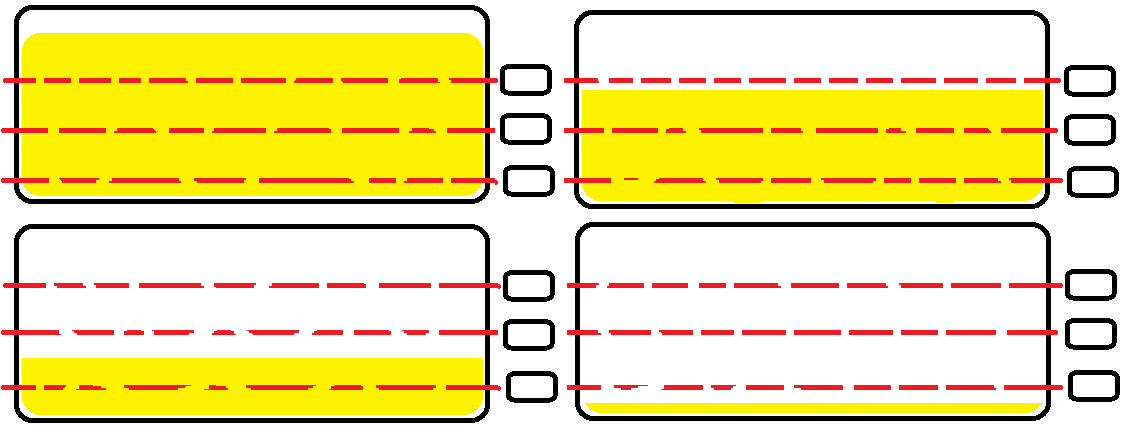
\includegraphics[scale=0.40]{img/infra1.png}
        \end{center}
	    \caption{Detección de alimento por niveles (Vista frontal del comedero).	
	    \label{infra1png}}
    \end{figure}
    
    Si el comedero se encuentra en un principio vacío (Estado de infrarrojos en 0), al momento de dosificar el alimento, los infrarrojos se encontrarán en un estado de 1. Una vez se cumpla el tiempo de espera para la ingesta del alimento, se corrobora si el estado de los sensores infrarrojos es nuevamente 0 (condición \#2).\\
    Si es así, la ingesta ha sido satisfactoria; en caso contrario se debe reportar en la base de datos y alertar inmediatamente al personal mediante un aviso correspondiente (sonoro, visual, etc). De esta manera se pueden satisfacer los objetivos específicos \#4 y \#5 al permitir la verificación de ingesta (satisfactoria/insatisfactoria) del alimento.
    
    
    
\subsection{Diseño}
% tornillo sin fin como extractor y transportador,
% El proceso de diseño para este subsistema abarca 3 partes. La primera consta de la conexión física y mecánica de las partes que comprenden el punto de dosificación. La segunda parte abarca el funcionamiento en conjunto del mecanismo de dosificación hasta el pesaje mediante la balanza digital. La última parte consta de una etapa de conexión entre el alimento pesado por la balanza y la entrega de ese alimento hasta el punto de alimentación del bovino (el plato). La tercera parte consta del diseño de la estructura física que soporta la parte tangible del sistema.\\

\subsubsection{Forma de la tolva}

En la sub-sección anterior se establece que la tolva debe ser a su vez el tanque de almacenamiento del cual se extrae el alimento, y que su ubicación debe estar en el establo de alimentación. En lo que respecta al diseño físico de este elemento, por simplicidad comercial  se opta por una tolva de forma cónica, también conocida como Silo (Ver figura \ref{tolvapng}).

\begin{figure}[H]
	\begin{center}
		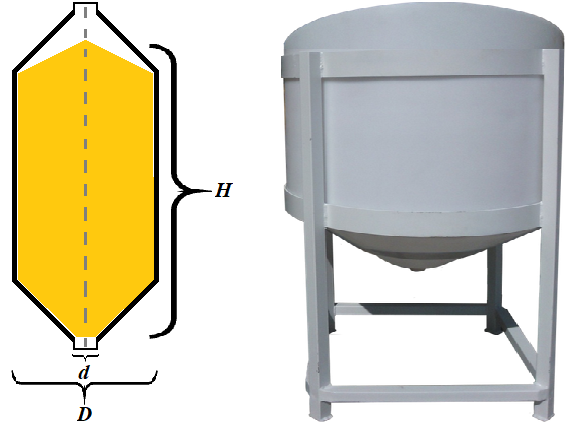
\includegraphics[scale=0.50]{img/tolvas.png}
	\end{center}
	\caption{Forma de la tolva. \label{tolvapng}}
\end{figure}

\subsubsection{Distribución de los puntos de alimentación}
Por otra parte, si se desea alimentar grupos de ganado de forma organizada y controlada, el tanque debe contar con un mecanismo tal que esté en la capacidad de abastecer a varios individuos a la vez. Para ello se diseñan puntos de alimentación en diferentes direcciones alrededor de cada tanque. De esta manera, 
%considerando las dimensiones físicas de ejemplares de esta ganadería,
se establecen hasta 4 puntos de alimentación por cada tolva instalada.
 
\begin{figure}[H]
	\begin{center}
		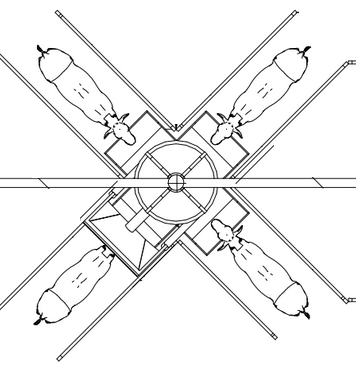
\includegraphics[scale=0.50]{img/disenotolvas.png}
	\end{center}
	\caption{Ubicación de la tolva. \label{matrizmotorpng}}
\end{figure}


% \subsubsection{Mecanismo de dosificación}

% El uso de tornillos sin fin exponen una dificultad práctica debido a su falta de disponibilidad directa en el mercado. Estos se fabrican acorde a las especificaciones del cliente, por lo tanto no es posible encontrar modelos que se adapten a las condiciones de trabajo ya establecidas. Como medida adaptativa a esta situación, se utiliza nuevamente la impresión 3D como alternativa viable para el desarrollo del prototipo y la validación del diseño que esta descrito a continuación.\\

\subsubsection{Mecanismo de extracción: Tornillo sin fin}\label{disenotorni}

Una desventaja comercial del tornillo sin fin es que solo se fabrican a la medida según la aplicación requerida; es por esto que éste debe ser diseñado con las especificaciones acordes a este proyecto para su fabricación a nivel comercial. Para hacer un diseño tentativo de éste, se realiza un modelo en 3D en SolidWorks.
%     \begin{figure}[H]
% 	\begin{center}
% 		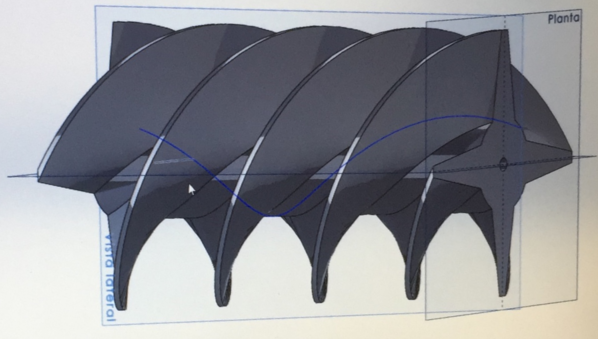
\includegraphics[scale=0.85]{img/torni3d.png}
% 	\end{center}
% 	\caption{Bosquejo 3D en SolidWorks del Tornillo sin fin. \label{torni3dpng}}
%     \end{figure}

Como se menciona en la sección \ref{endscrew}, el proceso de diseño de un mecanismo de dosificación mediante el uso de un tornillo sin fin consta de diferentes partes:

\begin{enumerate}[(1)]
    \item \textbf{Determinar el Paso ($P$), Diámetro interno ($d$) y Diámetro externo del tornillo ($D$): } Para acoplar el servomotor de giro continuo junto con el tornillo, se utiliza uno de los accesorios convencionales del servomotor (ver figura \ref{accesorioservopng}). Se utiliza este accesorio circular debido a que el tornillo consta de un diámetro interno, con eje rotativo concéntrico al eje giratorio del motor que le acciona, facilitando el acople entre ambas piezas.
    
    \begin{figure}[H]
	\begin{center}
		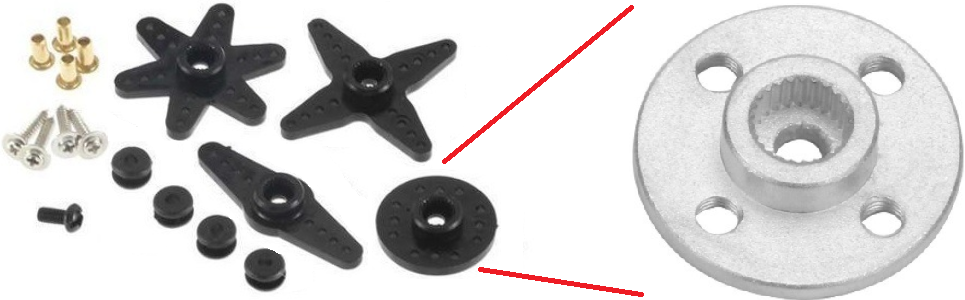
\includegraphics[scale=0.45]{img/accesorioservo.png}
	\end{center}
	\caption{Accesorios de rotación para servomotor. \label{accesorioservopng}}
    \end{figure}
    
    Este accesorio contiene 4 orificios por los que atraviesan 4 tornillos que por fricción conectan al accesorio y al tornillo. A grosso modo podría considerarse que la unión del accesorio y el tornillo conforman un accesorio más grande para el servomotor (ver Figura \ref{accesoriograndepng}).
    Para acoplar el accesorio del servo junto con el tornillo, el diámetro interno ($d$) de este último debe ser mayor o igual que el diámetro  externo del accesorio, es decir, aproximadamente una pulgada ($ 1 [inch] \approx 25,4 [mm]$).
    
    \begin{figure}[H]
	\begin{center}
		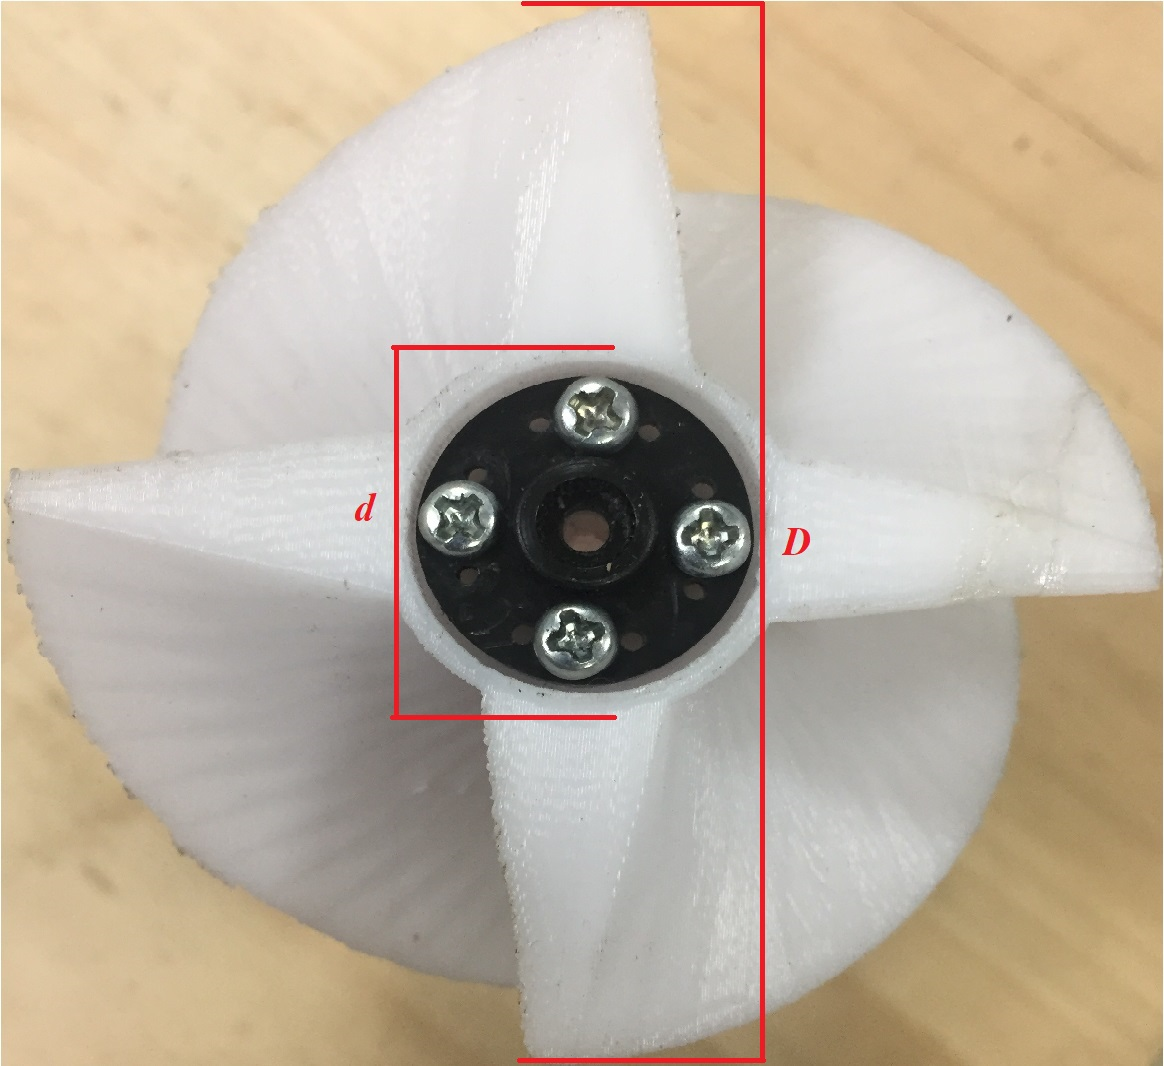
\includegraphics[scale=0.13]{img/accesoriogrande.png}
	\end{center}
	\caption{Accesorio ``tipo tornillo'' para servomotor. \label{accesoriograndepng}}
    \end{figure}
    
    Una vez establecido el diámetro interno del tornillo ($d$),  se considera por facilidad de diseño que el largo de las hélices serán de igual diámetro que $d$, dando como resultado que el Diámetro externo $D$ sea diseñado con un tamaño tres veces más grande que el interno ($ D = 3\cdot d $). No obstante, para garantizar que el tornillo girará sin inconvenientes ni roces forzosos o fricción indeseada con las paredes del canalón comercial de 3 pulgadas; se sustrae una holgura de $\pm 0,25 [mm]$ a cada lado dando como resultado que $D \approx 75 [mm]$.\\
    
    Como el material a transportar es pulverizado y semi granulado sólido, estos son considerados como materiales de buena capacidad de flujo. A su vez, las hélices deben ser continuas para garantizar el transporte continuo del material; por consiguiente basándonos en la tabla \ref{helices}, el paso ($P$) puede ser entre 1 a 2 veces el tamaño del diámetro interno $d$. Así pues, se considera un paso de igual tamaño que $d$.
    
    \item \textbf{Características del canalón y longitud del tornillo}
    
    Como ya se ha definido que el diámetro externo $D$ es $0,5 [mm]$ más pequeño que el diámetro interno del canalón, se puede confirmar que a esta nueva incógnita se le atribuye un valor de aproximadamente 3 pulgadas. Recapitulando lo explicado en la Sección \ref{endscrew}, el canalón es una superficie externa que bordea al tornillo de forma parcial o total, y a su vez hace parte de la armadura del mecanismo de dosificación.
    
    Comercialmente los tubos de PVC manejan dimensiones en pulgadas, facilitando su uso para este prototipo e incluso para aplicaciones reales. Con base en lo anterior el largo del canalón dependerá de las dimensiones comerciales de este producto.
    
    Entre las marcas más comerciales de tubería PVC están ``Pavco'' y ``Durman'', que poseen características y materiales similares. Sin embargo por motivos de limitantes económicos en este trabajo, se opta por los artículos menos costosos para las pruebas y/o modificaciones que se requieran.
    
    \begin{inparaenum}[(i)]
	        Antes de mostrar el tipo de tubería usada para representar el canalón, es imperativo observar que el canalón posee 3 aperturas de conexión hacia:
	        \item ``La tolva de almacenamiento'', mediante una boquilla de entrada de carga,
	        \item ``El motor de giro'' y por último
	        \item ``La salida del material'', mediante una boquilla de descarga.
	 \end{inparaenum}
	 
	 Con esto en mente, se opta por seleccionar una tubería tipo ``Tee'' como la que se muestra a continuación:
	 
	\begin{figure}[H]
	    \begin{center}
	    	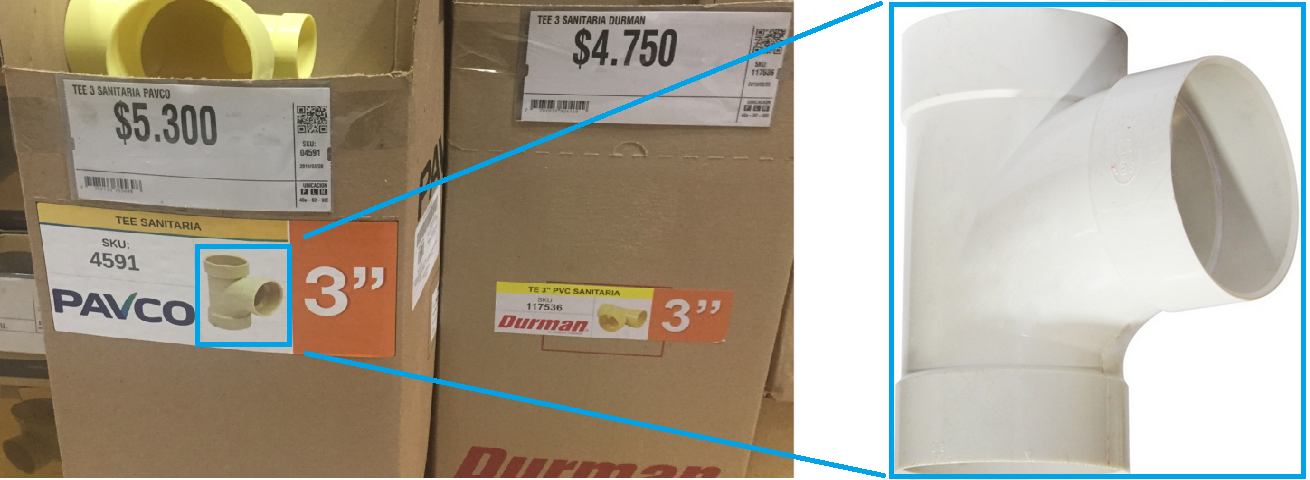
\includegraphics[scale=0.60]{img/pvct.png}
        \end{center}
	    \caption{Tubería de PVC tipo Tee. \label{pvctpng}}
    \end{figure}
	 
	De la figura \ref{pvctpng} se tiene que las aperturas opuestas conectarán con el motor y la boquilla de descarga respectivamente, mientras que la apertura restante conectará con la tolva de almacenamiento del alimento. 
	
	Antes de determinar el largo del canalón y por consiguiente el largo del tornillo, se debe agregar lo siguiente.
	
	Como la tubería de PCV tipo Tee no cuenta con una boquilla de descarga direccionada hacia abajo, se acopla un codo de ${90}^o$. Con esta añadidura se ayuda a guiar la caída del alimento pero esto requiere de una unión mediante un tubo de conexión para 3 pulgadas que ocasiona el alargamiento de la longitud final del canalón. 
% 	(ver figura 321654987). 
	
	En lo que respecta al extremo que conecta con el motor, se considera apropiado que para protegerlo y disminuir su exposición con el entorno, éste debe estar dentro de la armadura del sistema dosificador. De esta manera se añade un ``Adaptador para limpieza'' que conecta con la Tee sin necesidad de tubos de conexión (ver Figura \ref{adaptador3ppng}) y que además posee una tapa hermética que puede enroscarse y desenroscarse para acceder al motor en caso de reparaciones, manipulaciones, mantenimiento y limpieza en el futuro.
	
	\begin{figure}[H]
	    \begin{center}
	    	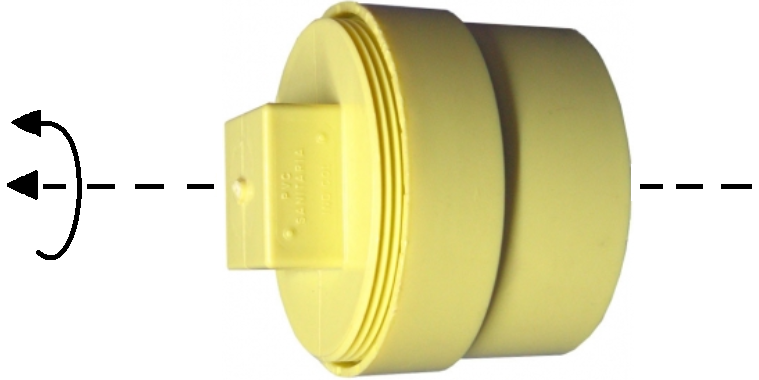
\includegraphics[scale=0.45]{img/adaptador3p.png}
        \end{center}
	    \caption{Adaptador para limpieza de PVC. \label{adaptador3ppng}}
    \end{figure}
	
	\pagebreak
% 	De igual forma para la apertura de conexión con el motor, se
    Finalmente se obtiene un canalón  compuesto  por el adaptador de limpieza, un tubo de conexión de $3"$, un codo de ${90}^o$ y la Tee de reducción de $3"$ a $2"$; que al unirlos  se obtiene que el canalón posee una longitud aproximada de $30 [cm]$.
    
    \begin{figure}[H]
	    \begin{center}
	    	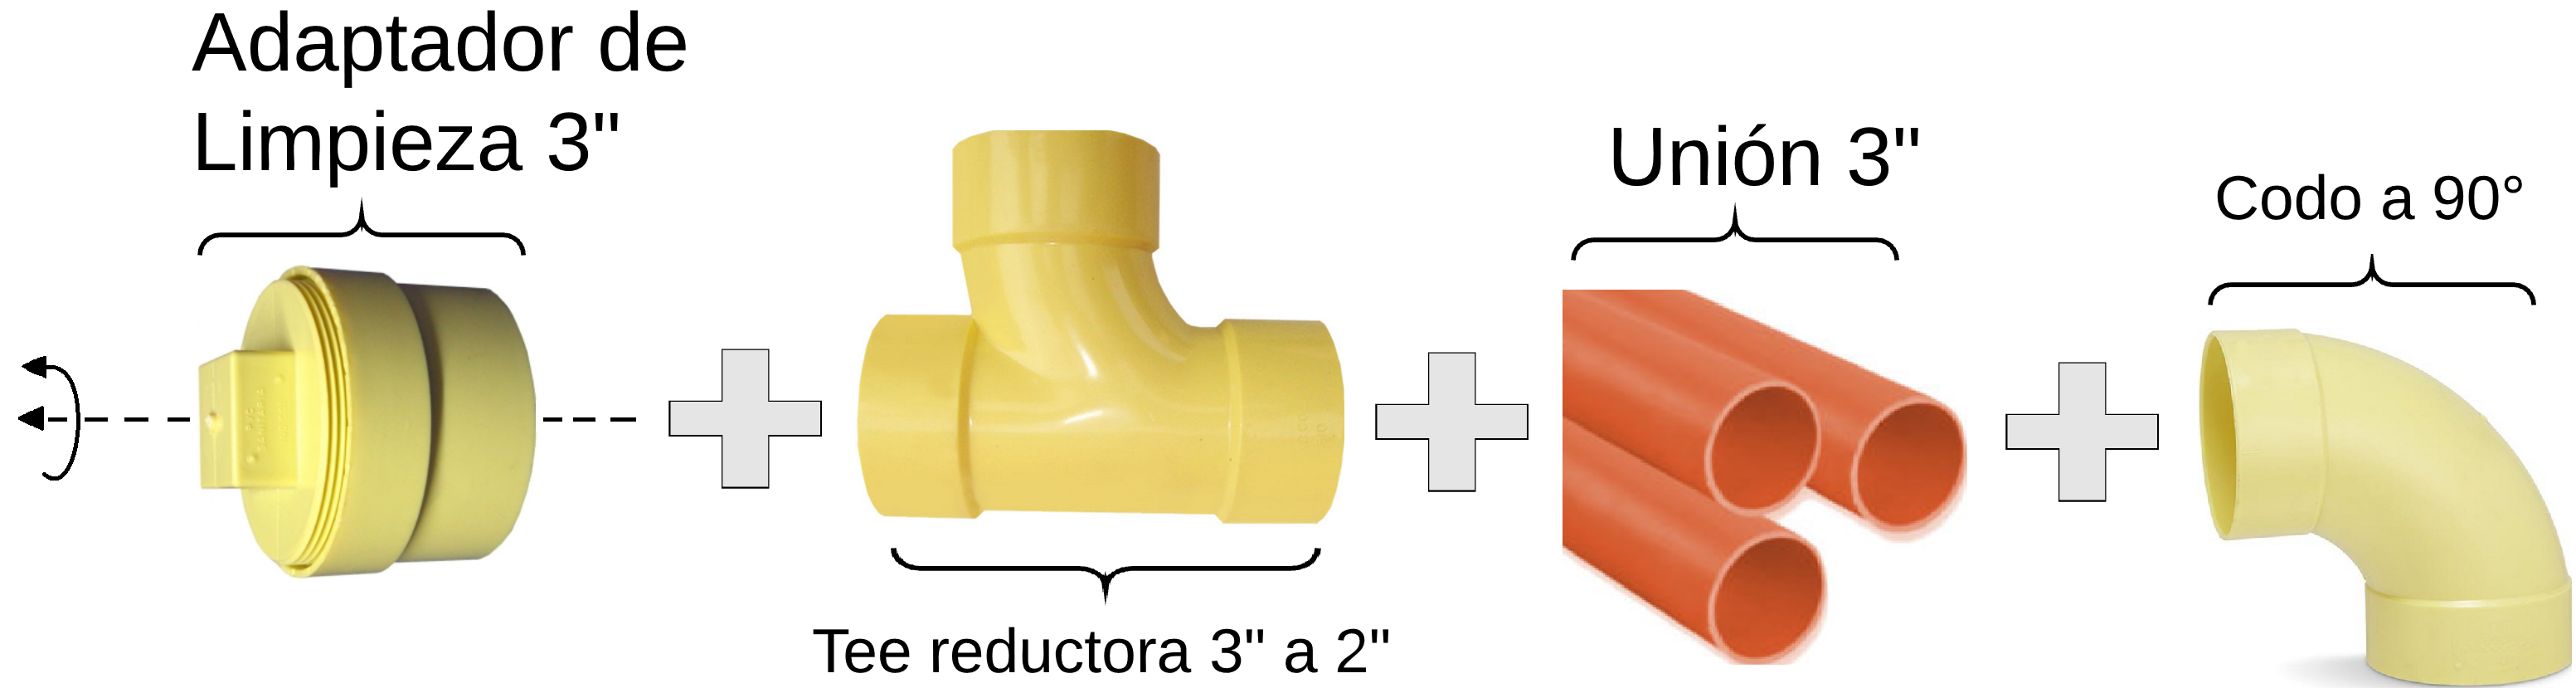
\includegraphics[scale=0.21]{img/canalontotal.png}
        \end{center}
	    \caption{Longitud total del Canalón. \label{adaptador3ppng}}
    \end{figure}
    
    Así pues, el tornillo al estar contenido dentro del canalón y al estar acoplado al motor de giro, poseerá una longitud menor a la longitud total del canalón. Se espera diseñar un Tornillo sin fin de $250[mm]$.\\
    
    \item \textbf{Diseño mecánico del tornillo sin fin}
    
    El diseño del tornillo parte del modelado en 3D. Este se realiza mediante la herramienta SolidWorks para el diseño, bosquejo, modelado y posibles modificaciones.
    Se parte del croquis de una superficie plana que será revolucionada para conformar un objeto final en 3D. Para esto, es importante establecer el número de hélices para dibujarlas en el croquis principal del transportador. En este caso, el tornillo será de $250[mm]$, por lo que se opta por tener 4 hélices equidistantes, de esta forma el croquis principal del tornillo obtiene la siguiente forma:
    
    \begin{figure}[H]
	    \begin{center}
	    	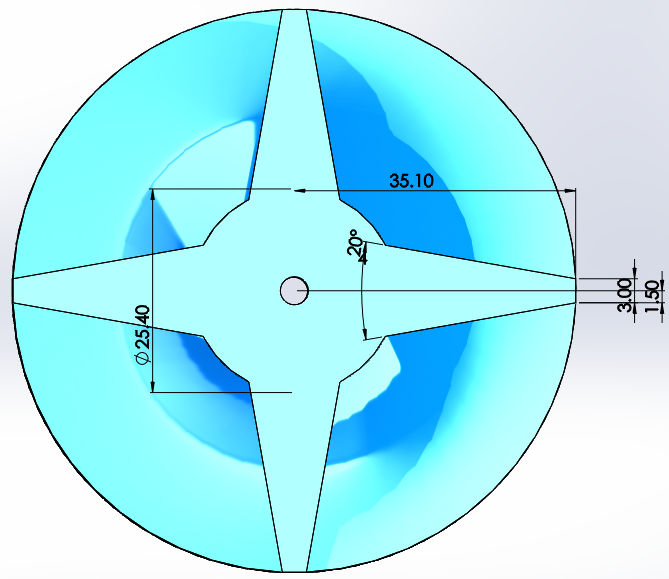
\includegraphics[scale=0.35]{img/croquisppal.png}
        \end{center}
	    \caption{Croquis principal del Tornillo sin fin. \label{croquisppalpng}}
    \end{figure}
    
    De esta forma, por cada revolución o vuelta completada por el tornillo se otorgarán 4 micro-dosificaciones (idealmente) de igual cantidad.
    Una vez definido el Croquis principal, se procede a utilizar la función de ``Barrido de saliente base'', con la que se revoluciona el croquis 2D conformando así el objeto 3D:
    
    \begin{figure}[H]
	    \begin{center}
	    	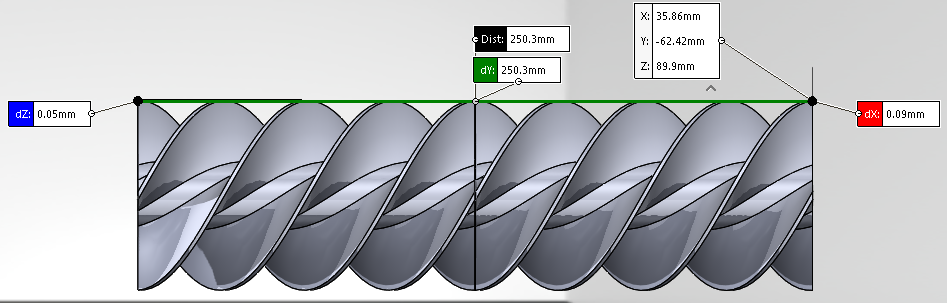
\includegraphics[scale=0.55]{img/largotorni.png}
        \end{center}
	    \caption{Primer Modelado de tornillo sin fin. \label{largotornipng}}
    \end{figure}
    
    \textbf{Obs: } Como se puede observar en la Figura \ref{croquisppalpng}, el tornillo diseñado cuenta con un orificio cuyo eje de rotación es concéntrico al eje de giro del motor y es por medio de este que se realiza el ajuste entre estas 2 partes. Para la elaboración del prototipo, se ajustará el accesorio ``Tornillo'', al espacio del motor de giro continuo mediante un tornillo de tipo M3 (ver figura \ref{torniservopng}).
    
    \begin{figure}[H]
	    \begin{center}
	    	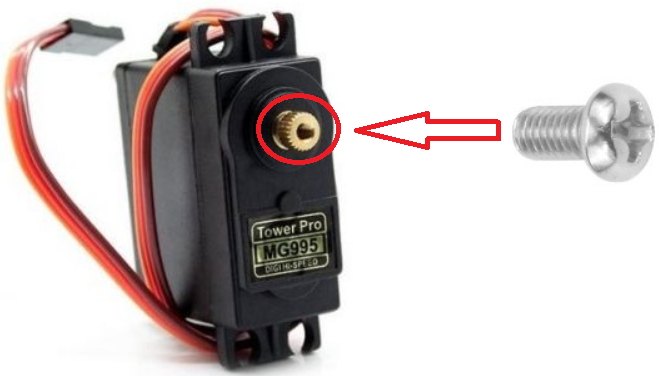
\includegraphics[scale=0.40]{img/torniservo.png}
        \end{center}
	    \caption{Tornillo de acople para accesorios del Servomotor. \label{torniservopng}}
    \end{figure}
    
    \end{enumerate}  % -------------------------------------------------------------
    \pagebreak
    \subsubsection{Mecanismo de  dosificación: Escobillas de barrido} \label{escobillas}
    
    Una vez finalizada la extracción de alimento y corroborado su peso, se debe trasladar el alimento desde la superficie de la balanza hasta la superficie del puesto de comida o en palabras técnicas, el comedero. Para ello se pensó en acoplar la balanza, a un mecanismo de giro que incline la misma y deje caer el alimento por gravedad (ver figura \ref{girobalanzapng}).
    
    \begin{figure}[H]
	    \begin{center}
	    	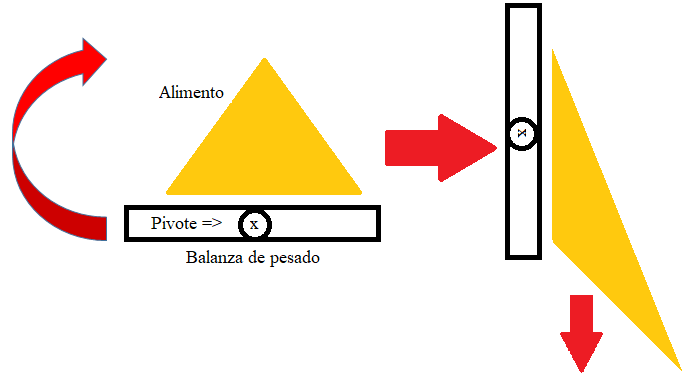
\includegraphics[scale=0.60]{img/girobalanza.png}
        \end{center}
	    \caption{Giro de la balanza. \label{girobalanzapng}}
    \end{figure}
    
    No obstante, el diseño comercial de las balanzas digitales posiciona la celda de carga de forma que el punto de presión esté en el extremo que hace contacto con la superficie de apoyo (mesa, piso) y no con la superficie que hace contacto directo con el material. Por lo tanto, si la presión ejercida sobre la balanza supera la presión soportada por el eje de giro usado para el movimiento rotativo de la balanza, no se podría realizar la inclinación de la balanza y el alimento no llegaría al plato de comida.  Como resultado, se opta por utilizar otra solución que satisfaga este último paso.
    
    Aunque los motores puedan usarse para mover objetos de forma lineal (directa o indirectamente), el movimiento básico de todo motor es el movimiento rotacional. Con base en esto se propone aprovechar esta característica para desplazar el alimento de la superficie de la balanza mediante escobillas de barrido que ``barran'' el alimento de la balanza. Así, si estas escobillas se encuentran acopladas a un motor de giro continuo, podrán barrer la porción de comida de manera continua. El diseño de esta pieza constará de 2 extremos que tendrán unida una superficie plana  para desplazar el alimento (en 1 y 2, Figura \ref{barredorespng}).

    \begin{figure}[H]
	    \begin{center}
	    	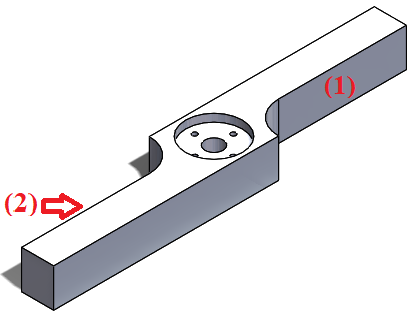
\includegraphics[scale=0.50]{img/barredores.png}
        \end{center}
	    \caption{Superficies para conexión de escobillas. \label{barredorespng}}
    \end{figure}
    
    En su centro se requiere de una hendidura para acoplarla con el motor de giro continuo al igual a como se hizo para el acople del tornillo sin fin (Ver Figura \ref{acopleservopng}).

    \begin{figure}[H]
	    \begin{center}
	    	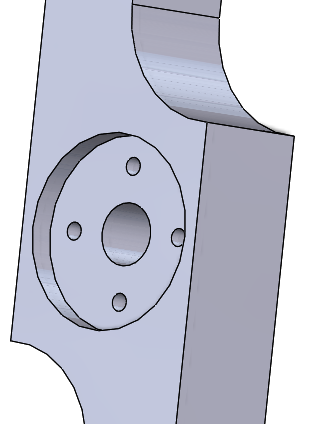
\includegraphics[scale=0.45]{img/acople_servo.png}
        \end{center}
	    \caption{Hendidura de acople para motor. \label{acopleservopng}}
    \end{figure}

    El diseño de un (1) accesorio de barrido se puede apreciar en la Figura \ref{vistasbarredorpng}, donde se puede observar  sus dimensiones en la vista inferior, seguido de la vista superior.
    
    \begin{figure}[H]
	    \begin{center}
	    	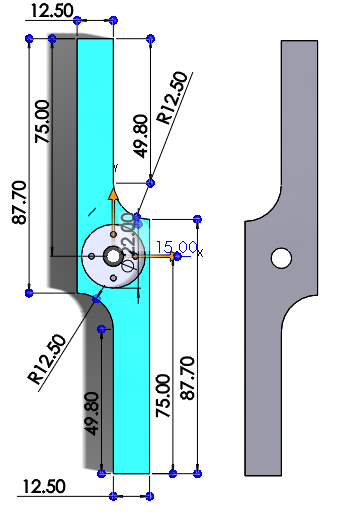
\includegraphics[scale=0.50]{img/vistasbarredor.png}
        \end{center}
	    \caption{Vistas Inferior, Superior del accesorio. \label{vistasbarredorpng}}
    \end{figure}

    Para garantizar el desplazamiento del alimento se hace uso de 2 motores a los lados de la balanza  y cada uno contará con una escobilla que al girar asincrónicamente desplazarán el alimento. 
    
     %---------------------------------------------------------------------------

    
    \subsubsection{Tipo de Comedero y detección de alimento}  \label{detectcomedero}

    Procediendo con el análisis previo de este ítem, si los sensores se ubican en una sola posición del plato se pueden presentar ocasiones en las que el alimento consumido se agrupe al extremo opuesto del sensor y se considere que el alimento ha sido ingerido satisfactoriamente cuando en realidad no es así (ver Figura \ref{infra2png}).

    \begin{figure}[H]
	    \begin{center}
	    	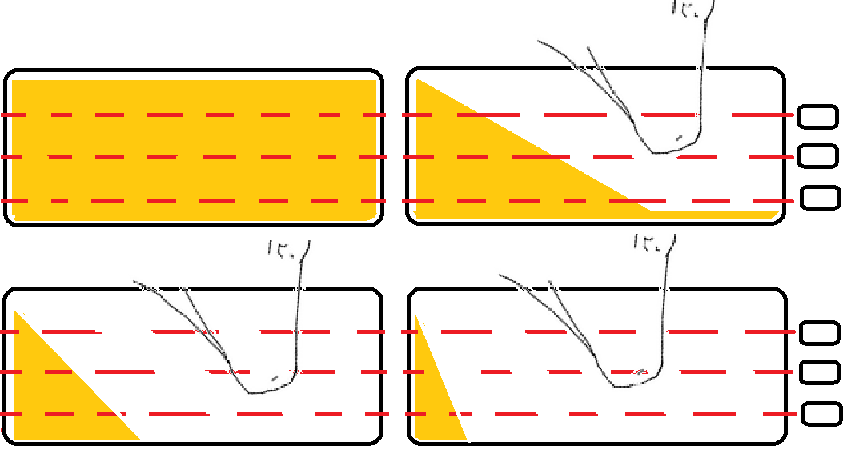
\includegraphics[scale=0.50]{img/infra2.png}
        \end{center}
	    \caption{Problema de detección \#1. \label{infra2png}}
    \end{figure}

    Como medida correctiva se opta por re-posicionar los infrarrojos en la base del plato, en forma de grilla circular, tratando de abarcar toda la superficie del comedero. No obstante se puede dar el caso que la grilla no abarque toda la superficie y se sigan presentando errores por no abarcar toda la superficie.
    % (ver vistas lateral y superior del comedero en la Figura \ref{infra3png}).

    \begin{figure}[H]
	    \begin{center}
	    	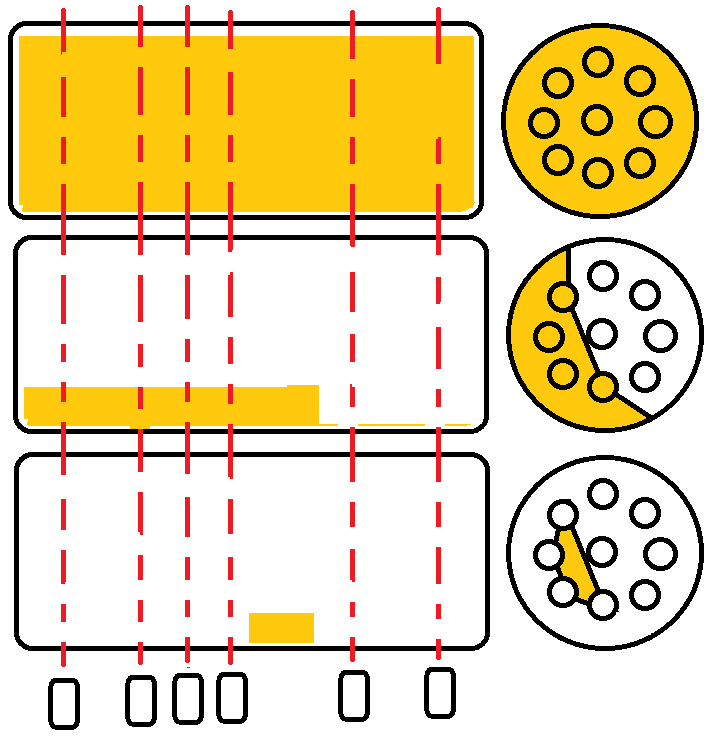
\includegraphics[scale=0.45]{img/infra3.png}
        \end{center}
	    \caption{Problema de detección \#2. \label{infra3png}}
    \end{figure}

    Así pues como última medida se opta por usar un comedero con detección vertical. De esta forma, a medida que el alimento es ingerido por el animal, éste seguirá cayendo por gravedad, así pues la grilla solo deberá ser posicionada en el extremo inferior del plato reduciendo el área de detección (Ver Vista lateral en la Figura \ref{infra4png}).
    
    \vspace{-200}
    
    \begin{figure}[H]
	    \begin{center}
    	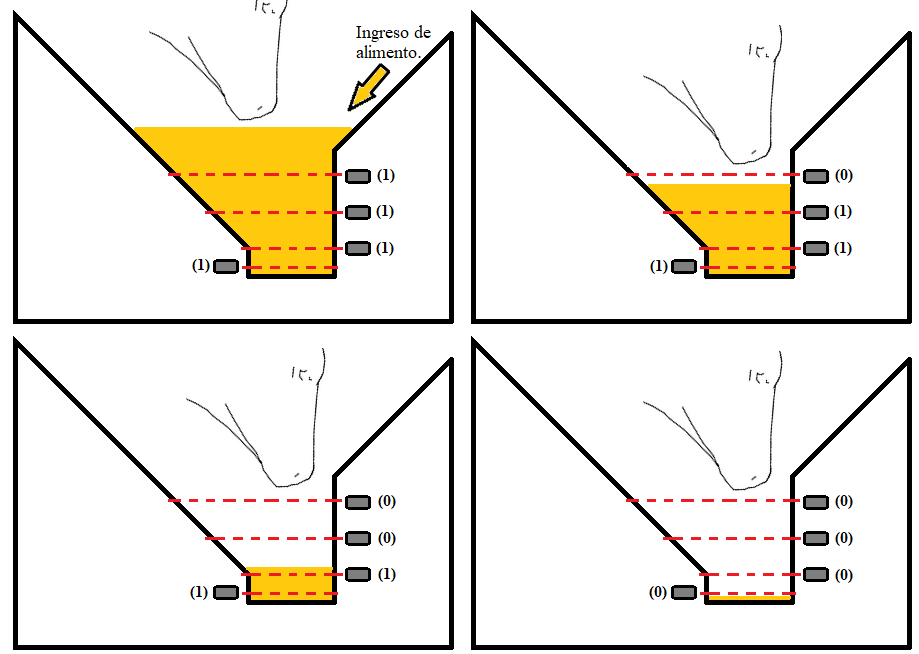
\includegraphics[scale=0.75]{img/infra42.png}
        \end{center}
	    \caption{Detección vertical de alimento en el comedero. \label{infra4png}}
    \end{figure}
    \pagebreak
    
    % \sout{hablar del diseño del suspensor del motor y de las escobillas como parte de la extracción y el pesado de alimentos y lo último de sistema de hardware hablar del plato y los infrarojos para detectar si comio o no el bovino y ahi acabo la seccion 5.3} (eso sin incluir al parte tangible la mesa, aunque eso creo que es mas un plus que algo imprescindible de hacer o de mencionar en el documento).
    
    % \textbf{Me falta cambiar las imágenes, caption y descripciones de las imagenes infra1,2,3 y 4} y paso al subsistema de sensores SECTION 5.4
    % \textbf{Me falta Agregar lo del tanque de almacenamiento y poner la figura uniones pvc que e sla que tiene todo el diagrama completo}
   
    
    % Improvise, Adapat, Overcome :)
    
    
   
    
    % ============================================
    % ============================================
    
    
     % Una vez llegados a este punto se procede a realizar la impresión 3D del tornillo en una de las impresoras 3D del CAP de la PUJ. No obstante se presentaron las siguientes dificultades:
    
    % \begin{itemize}
    %     \item La bandeja de impresión de las impresoras 3D del CAP solo imprime objetos de dimensiones menores a $140[mm]$.
    %     \item La longitud del tornillo diseñado supera esas dimensiones.
    %     \item El tiempo de impresión supera las 24 horas.
    %     \item El material requerido para hacer la impresión supera el monto autorizado para estudiantes de la carrera.
    % \end{itemize}
    
    % Estas limitaciones implican un rediseño del tornillo para que pueda ser impreso por lo que se toman las siguientes medidas:
    
    % \begin{itemize}
    %     \item El tornillo constará de 2 partes que al unirse conformarán el tornillo en su totalidad.
    %     % iguales que serán conectadas por 
    %     \item El diseño será modificado para que gaste menos material de impresión
    %     \item Al constar de diferentes piezas mas pequeñas se reduce el tiempo de impresión por pieza, ajustándose a la demanda de impresión del CAP.
    %     \item La longitud del tornillo será igual, pero las piezas que lo conforman tendrán dimensiones menores a $140[mm]$.
    % \end{itemize}
    
    
    % Retomando la figura \ref{accesoriograndepng}, el diseño de uno de los extremos del tornillo debe contener los orificios necesarios para realizar el acople entre el servo y el tornillo. Este diseño se puede apreciar a continuación:
    
    % \begin{figure}[H]
	   % \begin{center}
	   % 	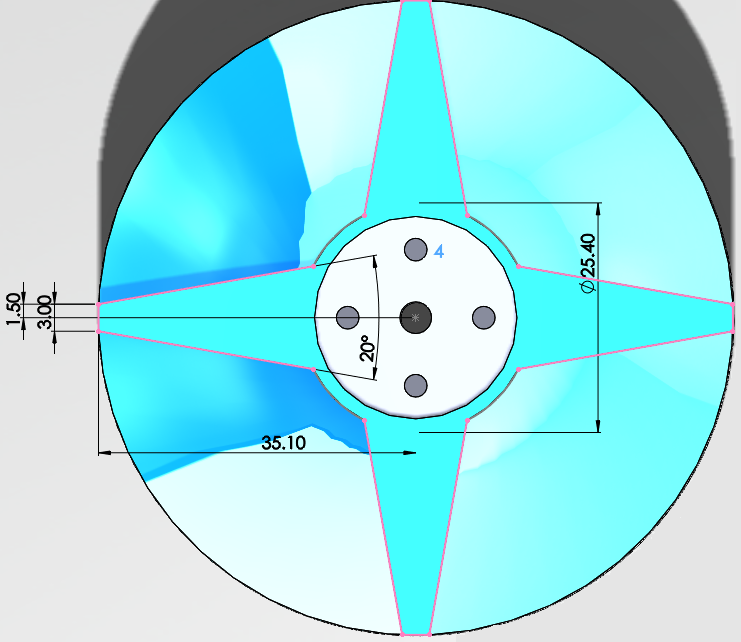
\includegraphics[scale=0.5]{img/motornillo.png}
    %     \end{center}
	   % \caption{Diseño del extremo del Tornillo que conecta con el servo motor. \label{motornillopng}}
    % \end{figure}
    
    
    % Ahora bien, dado que el tornillo constara de 2 partes, se debe considerar el modo de conexión. Para ello se opta por diseñar una parte tipo ``Macho'' y otra parte tipo ``Hembra''. De esta forma, el tornillo completo estaría formado por la conexión a presión de ambas partes.
    
    % \begin{figure}[H]
	   % \begin{center}
	   % 	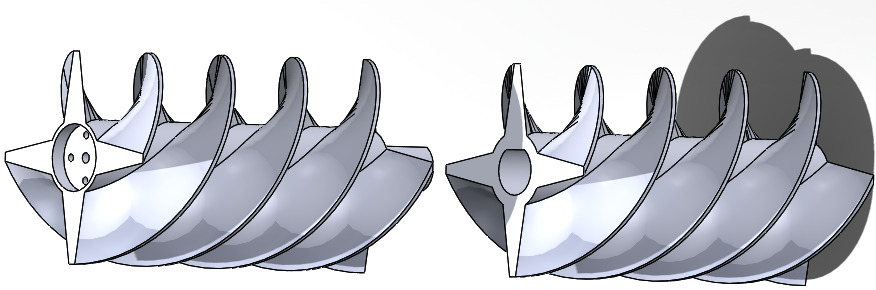
\includegraphics[scale=0.6]{img/semicircular.png}
    %     \end{center}
	   % \caption{Unión entre tornillos tipo ``Hembra'' y tipo ``Macho''. \label{semicircularpng}}
    % \end{figure}
    
    % Se había pensado que con la saliente semicircular del tornillo Macho sería suficiente para transmitir de manera apropiada el torque desde el servo hasta el extremo del tornillo. No obstante, el tornillo se ``desacoplaría'' en las condiciones en que el tornillo esté en su máxima capacidad de transporte, es decir cuando el tornillo este transportando alimento desde su inicio hasta su fin. 
    
    % De esta forma se concluye que no se ejerce fricción suficiente entre las paredes internas del tornillo que bordean la saliente del tornillo Macho y de esta forma no se transmitiría de manera apropiada el torque desde el servo hasta el extremo final del tornillo.
    
    % Con base en lo anterior, se concluye que es necesario el uso de una $3^{er}$ pieza de conexión. Esta pieza deberá tener superficies planas que ayuden a la transmisión de torque. Por otra parte debe estar separado de ambos extremos por efectos de impresión y de calentamiento del material.\\
    
    
    % Siguiendo este orden de ideas, se resume lo siguiente:
    % \begin{itemize}
    %     \item El tornillo constará de 2 partes.
    %     \item La primera que conecta el servo junto con un extremo del tornillo
    %     \item La segunda que conecta, mediante una pieza extra, las 2 partes del tornillo.
    %     \item Ambas partes del tornillo serán de tipo ``Hembra''.
    %     \item La pieza de conexión contará con 2 orificios que servirán para pasar un seguro que mantendrá firme el acople de las 2 partes de tornillos con la pieza de conexión. (ver figura \ref{piezaconexionpng})
        
    %     \begin{figure}[H]
	   %     \begin{center}
	   % 	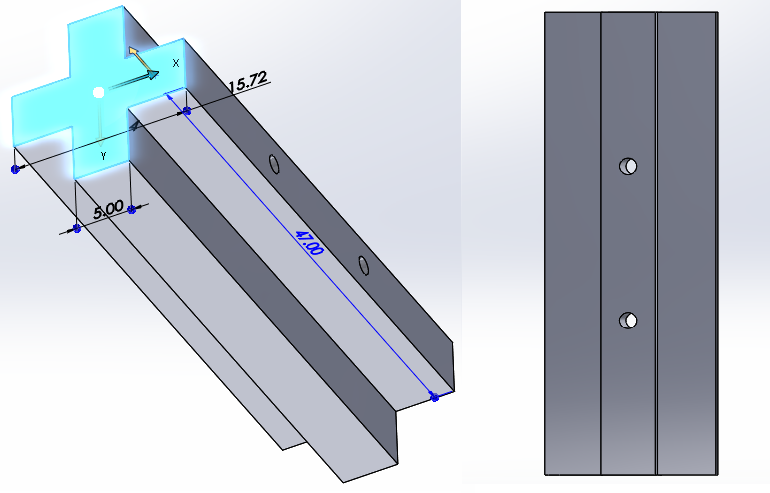
\includegraphics[scale=0.5]{img/piezaconexion.png}
    %         \end{center}
	   %     \caption{Pieza auxiliar para conexión del Tornillo. \label{piezaconexionpng}}
    %     \end{figure}
        
    %     \item Ambas piezas de tornillo tipo Hembra tendrán un orificio sobre el eje principal basados en el ítem anterior.
    % \end{itemize}
    
    % En este punto se podría cuestionar la estructura interna del tornillo debido a la dificultad visual para asimilar el diseño del tornillo. Para ello se muestra el siguiente corte trasversal de la pieza de tornillo Hembra que conecta  con el servomotor (ver figura \ref{cortetrasversalpng})
    
    % \begin{figure}[H]
	   % \begin{center}
	   % 	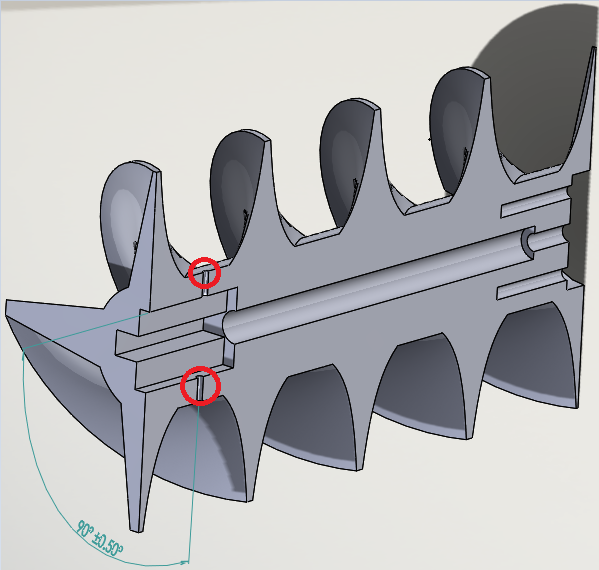
\includegraphics[scale=0.55]{img/cortetrasversal3.png}
    %     \end{center}
	   % \caption{Corte trasversal pieza tipo Hembra. \label{cortetrasversalpng}}
    % \end{figure}
    
    % \vspace{1mm}
    
    
    % En el lado izquierdo de la figura \ref{cortetrasversalpng} se puede observar el espacio para unir la pieza de conexión y el seguro. En la parte media de la figura se puede observar el corte interno del tornillo por donde pasa el atornillador que fija el tornillo M3 al servo. Por último, en el lado derecho se observa los 4 orificios para atornillar el accesorio circular del servo a la pieza del tornillo. \\
    
    % Adicionalmente se puede observar la vista superficial de esta pieza tipo Hembra en la figura \ref{vistainternapng}.
    
    % \begin{figure}[H]
	   % \begin{center}
	   % 	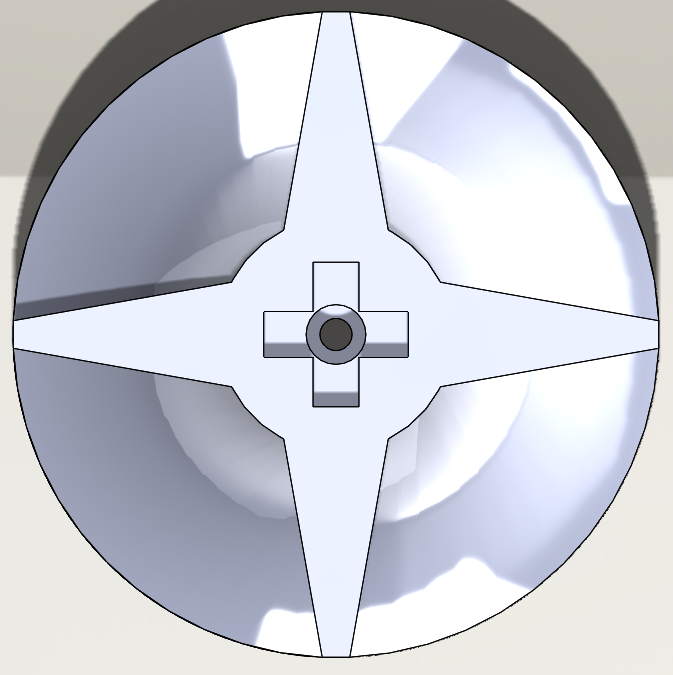
\includegraphics[scale=0.5]{img/vistainterna.png}
    %     \end{center}
	   % \caption{Vista interna de pieza tipo Hembra. \label{vistainternapng}}
    % \end{figure}
    
    % La composición final del tornillo consta del ensamblaje de las 2 piezas tipo hembras y el conector tipo cruz. el ensamblaje se logra al unir estas piezas como lo indica la figura \ref{ensambletornipng}:
    
    % \begin{figure}[H]
	   % \begin{center}
	   % 	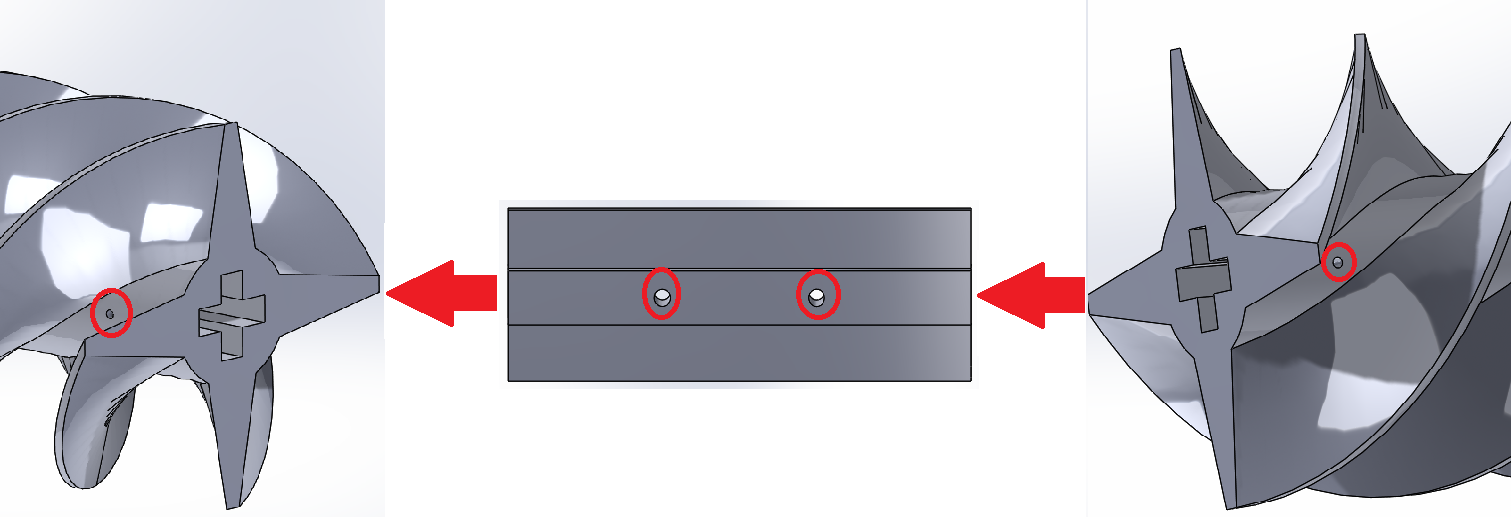
\includegraphics[scale=0.35]{img/ensambletorni.png}
    %     \end{center}
	   % \caption{Ensamble del tornillo. \label{ensambletornipng}}
    % \end{figure}
    

    % \item \textbf{Pesaje de porción: }
    
    % En lo que respecta al pesaje de la porción de alimento se ha preestablecido que ésta sería pesada a medida es extraída del tanque de almacenamiento para corroborar la cantidad ($en gramos$) que se entregará al bovino correspondiente. Para ello se requiere de una herramienta que permita medir peso. Los sensores especializados para este tipo de mediciones son las galgas extensométricas o las celdas de carga (ver figura \ref{celdaspng}). Mediante estas, se puede medir la presión que ejerce un objeto sobre una superficie y de esta forma se puede calcular la masa ([$g,kg,...$]) del objeto.
    % \begin{figure}[H]
	   % \begin{center}
	   % 	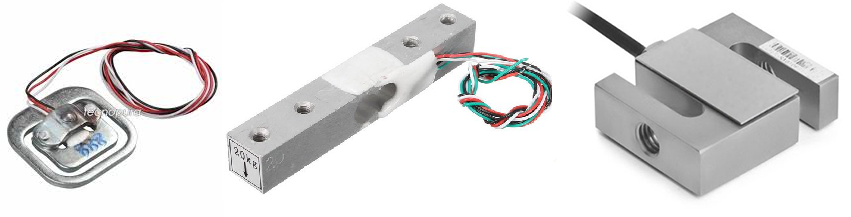
\includegraphics[scale=0.80]{img/celdas.png}
    %     \end{center}
	   % \caption{Celdas de carga y galga extensométrica. \label{celdaspng}}
    % \end{figure}
    % Estos dispositivos requieren de un acondicionamiento de la señal mediante un puente de ``Wheastone'' y de un sistema mecánico que permita distribuir la fuerzas de manera proporcional sobre toda la superficie de contacto. Además, para entregar los datos de manera digital se requiere de una etapa de conversión por medio de un ADC.
    % No obstante, en cuestión de recursos económicos, tiempo y facilidad de uso, resulta más fácil utilizar una balanza digital comercial que fabricar una balanza desde cero. De esta forma se puede aprovechar el diseño mecánico y la ubicación del sensor y solo resta transformar la señal analógica a digital.  Para esta última tarea, se utiliza el chip HX711 que  incluye el puente de ``Wheastone'' junto con una etapa de amplificadora y el ADC simplificando significativamente la inclusión de circuitería. 
    
    % A modo general, la etapa encargada de pesado el alimento extraído del tanque se observa en la figura \ref{pesajepng}:
    
    % \begin{figure}[H]
	   % \begin{center}
	   % 	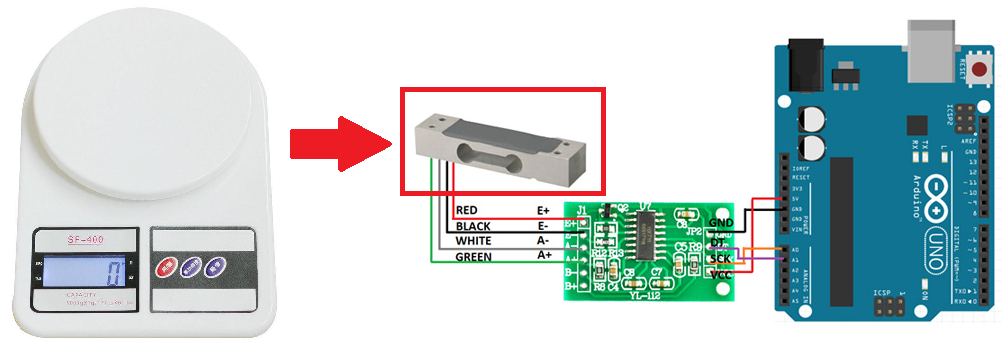
\includegraphics[scale=0.70]{img/pesaje.png}
    %     \end{center}
	   % \caption{Medición general del peso. \label{pesajepng}}
    % \end{figure}
    
    % ============================================
    % ============================================
    

\pagebreak
\section{Subsistema de Hardware} \label{subsissen} 

El subsistema de Hardware comprende los elementos electrónicos encargados de medir variables, acondicionar las señales analógicas y transformarlas en digitales. También se incluye a los elementos electrónicos y/o electromecánicos usados para accionar los elementos mecánicos del prototipo descritos en las Sección \ref{subsishw}. Siguiendo este orden de ideas, se procede de la siguiente manera:

\subsection{Sensado}

Para este prototipo se desea medir variables referentes a la iteración de Ceba que sirvan para monitorear la evolución alimenticia de cada bovino de manera individual. Con este objetivo en mente y teniendo en cuenta lo explicado en los 2 subsistemas ya descritos, se requieren de las siguientes etapas electrónicas de sensado:

\subsubsection{Nivel de alimento de la tolva}\label{lvltolva}
Para corroborar que se cuenta con suficiente comida para abastecer a el(los) próximo(s) grupo(s) de ganado, se necesita verificar el nivel de alimento del tanque. Desde el punto de vista electrónico, esto puede lograrse gracias a diferentes sensores de nivel dependiendo del tipo de fluido almacenado. No obstante al tener acceso a las porciones dietarias del ganado, la densidad y la altura que ocupa esta cantidad dentro de la tolva, se puede estimar la cantidad total mínima requerida ($Cant_{Min}$). De esta manera se puede calcular una cantidad existente dentro el tanque a medida que se dosifican las porciones.
% De esta manera se plantea utilizar una detección similar a la ya descrita en la Sección \ref{detectcomedero}.

Es importante notar que la cantidad total de alimento requerido es dinámica en una aplicación real, por lo tanto no es sencillo determinar un monto mínimo. Sin embargo, se puede estimar un monto de ejemplo en ``el peor de los casos''. Esta situación se presupone de la siguiente manera:

\begin{enumerate}[(i)]
    \item Todos los bovinos son similares.
    \item Todos poseen un peso aproximadamente igual.
    \item Todas las reses estabuladas están próximas a alcanzar el peso ideal.
    \item Se tiene conocimiento de la capacidad máxima de almacenamiento.
    \item El re abastecimiento del tanque de alimento se realiza hasta el valor máximo permitido en el tanque (item anterior).
    \item Se tiene conocimiento del peso máximo ideal.
    \item En caso que no se conozca el peso máximo ideal, se considera un valor de $600[kg]$.
    \item El valor anterior es un valor máximo  de referencia comercial para excelentes ejemplares (muy poco común en el rango de edad de la Ceba).
\end{enumerate}

Basados en la información anterior, se procede a calcular la porción mínima requerida para esta situación:

% \begin{enumerate}[(i)]
    Retomando lo explicado en el Capítulo \ref{cap3}, un ejemplar debe consumir lo equivalente a un 10\% de su peso actual; de esta forma la cantidad total de dieta consumida por cada bovino será de $Alimento_{Total} = 60[kg]$.
    La porción de alimento dietario de un ejemplar está entre un 10 y un 20\% del alimento, por lo que en esta situación se considera un 20\%. Dando como resultado una cantidad de $Alimento_{Dieta} = 12[kg]$ por cabeza.
    Así pues la cantidad mínima requerida en el tanque se obtendría de la siguiente manera:

    \begin{equation}
        Cantidad_{Min} = \frac{\left(Cantidad_{Reses}\cdot Alimento_{Dieta}\right)}{Cantidad_{Tolvas}}. \label{ecuaminima}
    \end{equation}
% \end{enumerate}

Ahora bien, en una implementación a escala real de lo diseñado en este proyecto se considera una situación hipotética con una cantidad total de 12 reses, una cantidad total de 3 tolvas; y por consiguiente el resultado para la ecuación \ref{ecuaminima} es:  

    \begin{equation}
        Cantidad_{Min} = \frac{\left(12\cdot 12[kg]\right)}{3} = 48[kg]. \label{ecuaminima2}
    \end{equation}
% \end{enumerate}

Teniendo en consideración la relación de escala (100:1) para la validación del prototipo (mencionada en \ref{limites}), el resultado de la ecuación \ref{ecuaminima2} es:

\begin{equation}
    Cantidad_{Min} = \frac{48000[g]}{100} = 480[g]. \label{ecuaminima3}
\end{equation}

% opc 1
% Para este caso hipotético de validación del prototipo, esta cantidad representa una altura $h$ en la tolva y es por medio de ésta que se puede utilizar una detección similar a la ya mencionada en la sección anterior. Si la altura de alimento en la tolva $H_t$ disminuye por debajo de la altura $h$ significa que el alimento no será suficiente para dar abasto a un próximo ganado entrante. Así pues se da solución al objetivo específico No. 1 de la Sección \ref{objesp}.\\

% opc2
Para validar el prototipo en esta situación hipotética, se puede verificar el alimento existente del tanque mediante una variable acumuladora que se substrae del valor máximo almacenado en el tanque al final de una jornada de dosificación, dado que se considera que se ha re abastecido en su totalidad. Esta variable ira acumulando las dosis que se han dosificado y en caso tal que el alimento neto del tanque (ecuación \ref{ecuaneto}) sea menor a la cantidad mínima (ecuación \ref{ecuaminima3}) se da aviso para su re abastecimiento.\\

\vspace{-25}
\begin{equation}
    Cantidad_{Neta} = Cantidad_{Max Tanque} - Cantidad_{Servida Acumulada}[g] .  \label{ecuaneto}
\end{equation}

Una segunda opción puede ser que la cantidad mínima representa una altura $h$ en la tolva y es por medio de ésta que se puede utilizar una detección similar a la ya mencionada en la sección anterior. Si la altura de alimento en la tolva $H_t$ disminuye por debajo de la altura $h$ significa que el alimento no será suficiente para dar abasto a un próximo ganado entrante. Así pues se da solución al objetivo específico \# 1 de la Sección \ref{objesp}.\\

% \textbf{*------   Bitácora del tiempo de PIPE 15/11/19: Me quedé aqui   -----*}\\

\subsubsection{RFID}

Para lo concerniente a la identificación de ganado, los dispositivos encargados de cumplir esta tarea son los RFID tag de las Jáquimas RFID de la sección \ref{subsisid}, y su funcionamiento en conjunto con los lectores RFID del Capítulo \ref{cap4}.

\subsubsection{Pesaje de alimento / Pesaje de Bovino}

Para solventar el objetivo específico No. 7 y complementar el objetivo específico No. 2, tanto el pesaje del alimento dosificado como el pesaje de las reses se pueden lograr mediante el mismo principio con el uso de los mismos tipos de sensores solo que con diferente capacidad de medida.

A modo general, la medición de un peso se logra mediante el uso de celdas de carga. Estas varían en forma y tamaño (ver Figura \ref{celdaspng}), dependiendo de la carga total a la que están expuestas. Mediante estas, se puede medir la presión que ejerce un objeto sobre una superficie y de esta forma se puede calcular la masa total del objeto ($[g], [kg], ...$).

    \begin{figure}[H]
	    \begin{center}
	    	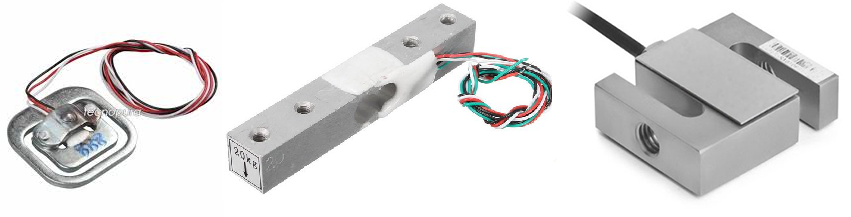
\includegraphics[scale=0.80]{img/celdas.png}
        \end{center}
	    \caption{Diferentes tipos de celdas de carga. \label{celdaspng}}
    \end{figure}

    Estos dispositivos requieren de un acondicionamiento de la señal analógica mediante un puente de ``Wheatstone'' y de un sistema mecánico que permita distribuir la fuerzas de manera proporcional sobre toda la superficie de contacto. Además, para entregar los datos de manera digital se requiere de una etapa de conversión por medio de un ADC.
    En cuestión de recursos económicos, tiempo y facilidad de uso, resulta más fácil utilizar una balanza digital comercial que fabricar una balanza desde cero. De esta forma se puede aprovechar el diseño mecánico y la ubicación del sensor y solo resta transformar la señal analógica a digital.
    
    En cuestión del prototipo, se utiliza el chip HX711 que incluye el puente de ``Wheatstone'' junto con una etapa de amplificación y el ADC simplificando significativamente la inclusión de circuitería.
    
    \begin{figure}[H]
	    \begin{center}
	    	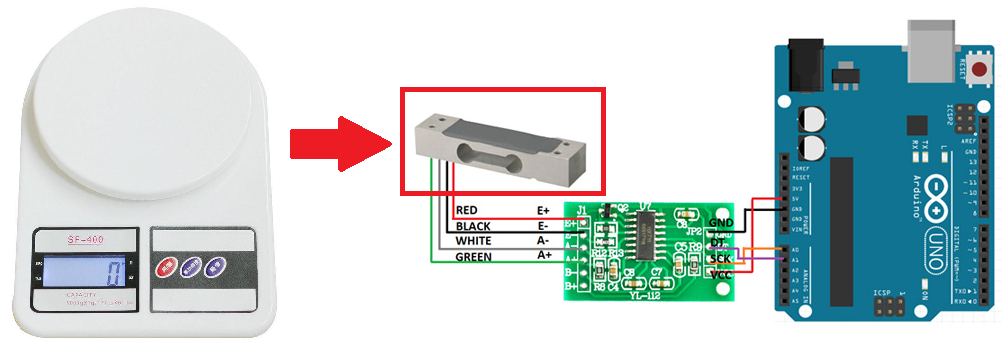
\includegraphics[scale=0.70]{img/pesaje.png}
        \end{center}
	    \caption{Medición general del peso. \label{pesajepng}}
    \end{figure}
    
    A modo general, el sistema electrónico encargado de pesar el alimento extraído del tanque y/o de adquirir el peso actual de un bovino (según corresponda) se observa en la Figura \ref{pesajepng}.
    % \textbf{CAMBIAR LA CELDA Y EL HX POR UN BLOQUE WHEATSTONE Y ADC}:

%%% Tek

% \subsubsection{TEMPORIZADOR}
% \subsubsection{Peso Balanza 2}
\subsubsection{Detección de alimento en el comedero}

Como se explicó en la Sección \ref{detectcomedero}, la detección de cantidad de alimento ingerido satisfactoriamente se logra si se cumplen 2 condiciones transitorias, ayudadas por un temporizador cuyo valor puede ser fijado por el productor ganadero. La detección de alimento se realiza mediante sensores infrarrojos ubicados en el costado vertical del comedero cuya distribución se puede apreciar en la Figura \ref{infra4png}.

\subsection{Actuadores}
\subsubsection{Motor de giro continuo}\label{mg995}

Como se mencionó antes, tanto el tornillo sin fin como las escobillas de barrido, son los elementos encargados de dosificar mecánicamente el alimento extraído desde la tolva y entregada en el comedero. No obstante, estos accesorios requieren de un dispositivo eléctrico para que puedan ejecutar su finalidad. Estos accesorios cumplen su papel mediante movimientos rotativos, realizados por motores DC de giro continuo.\\

Se considera pertinente dar prioridad a los servomotores que a otras modalidades, por su facilidad de uso, alimentación y manipulación mediante señales de control, reduciendo el uso de sistemas complejos como los requeridos para el uso de motores de alta potencia como los motores paso a paso.

Es importante recalcar el hecho que los motores deben estar en capacidad de garantizar un giro continuo para satisfacer el accionamiento mecánico del tornillo y de las escobillas de barrido, por lo que deben usarse motores especiales para $360^{o}$ de giro.
Por último, el motor debe estar en la capacidad de transmitir el torque necesario para girar su carga respectiva, por lo que en este caso, el motor debe contar adicionalmente con altas capacidades de torque.\\

En cuestión de prototipado de este proyecto, los servomotores de giro continuo usados son los $Tower Pro  MG995$ con una capacidad de torque a $5[V]$ de $9.4\left[\frac{kg}{cm}\right]$. Cuentan con engranaje metálico y pueden ser acoplados a otros accesorios externos mediante tornillos M3.

\begin{figure}[H]
    \begin{center}
    	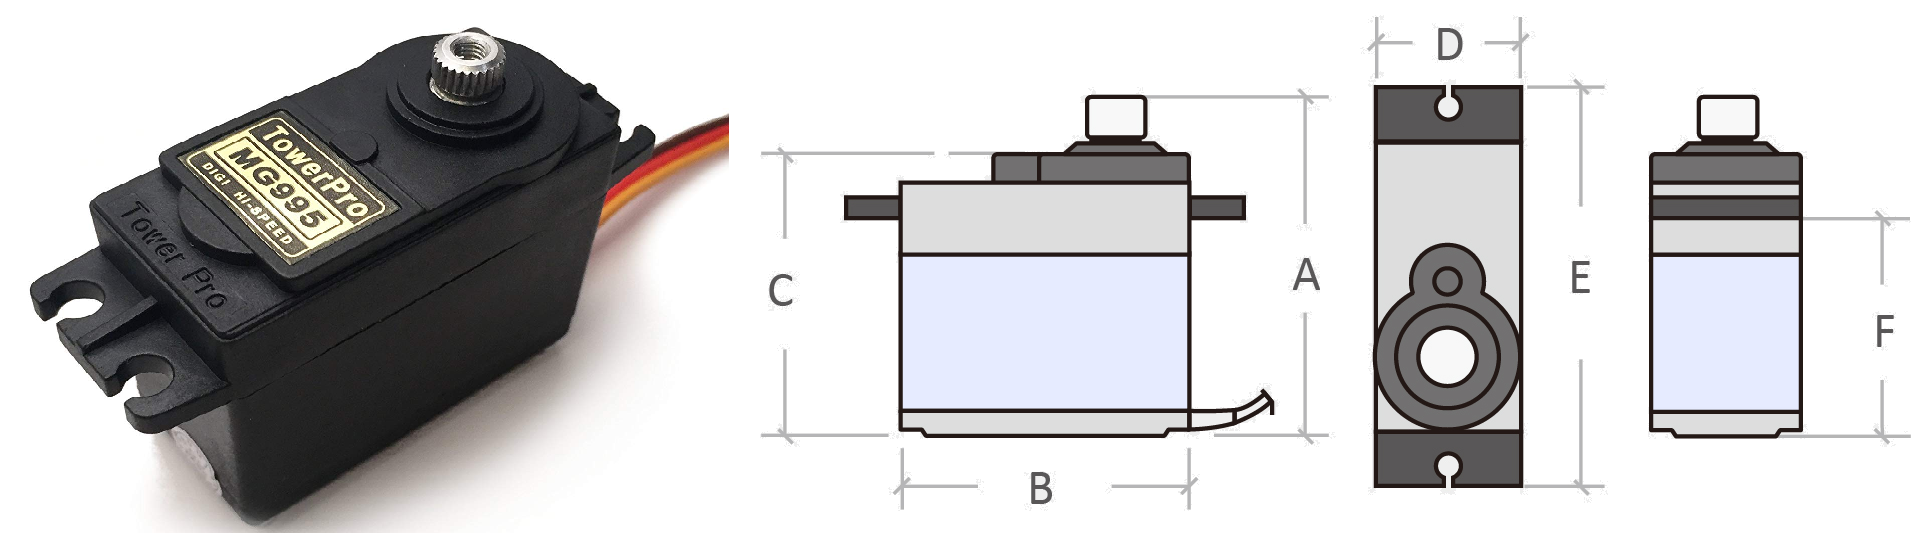
\includegraphics[scale=0.35]{img/servopro.png}
    \end{center}
    \caption{Servomotor de giro continuo TowerPro MG995. Tomada de \cite{servopro} \label{servopropng}}
\end{figure}

Donde $A=42.7[mm], B=40.9[mm], C=37[mm], D=20[mm], E=54[mm], F=26.8[mm]$.

\subsubsection{Sistema de Alarmas}

Aún cuando un sistema pueda ser diseñado con el objetivo de abarcar la mayoría de los posibles comportamientos, todo sistema está sujeto a posibles fallas o comportamientos indeseados. En este caso, para el desarrollo de este proyecto no se desean algunos comportamientos como los siguientes:

\begin{enumerate}
    \item Los bovinos ingieran su alimento de manera incorrecta,
    \item Se dé el caso que una res intente consumir más cantidad de alimento del especificado,
    \item Se agote el alimento a dosificar,
    \item Se ingresen animales no identificados,
    \item Entre otros.
\end{enumerate}

Para cuando se presenten estos casos indeseados se espera poder dar aviso al personal ganadero pertinente, por lo que se plantea el uso de diferentes alarmas como por ejemplo alarmas sonoras o alarmas visuales. Para el desarrollo del prototipo, se hará uso de alarmas visuales mediante un arreglo de diodos LED, y de alarmas sonoras mediante buzzers o pequeños altavoces.

\subsection{Microcontrolador}

Este proyecto está orientado al uso de dispositivos de manipulación de sensores y actuadores de bajo costo como los microcontroladores mencionados en el Capítulo \ref{cap4}. Estos serán los dispositivos encargados de recibir los datos sensados junto con los parámetros de entrada entregados por el productor ganadero (Usuario). También están encargados de procesar los datos y hacer la activación de los actuadores respectivos según sea el caso. Finalmente realizan el registro de los datos correspondientes en la(s) base(s) de datos. Como posibilidad adicional pueden ser conectados a dispositivos de representación gráfica o a interfaces gráficas de usuario (GUI) (\textit{\textbf{No incluidas dentro de los alcances de este proyecto}})

En este proyecto, se utiliza un Arduino Mega. Este microprocesador facilita la prueba del prototipo debido a su gran variedad de pines analógicos y digitales con lo que se puede lograr una conexión completa de los dispositivos a utilizar sin la necesidad de módulos externos o módulos adicionales.

% \pagebreak
% \subsubsection{Arduino}

% \subsection{MicroProcesador}
% \subsubsection{Arduino}

%  \item \textbf{Pesaje de porción: }
    
%     En lo que respecta al pesaje de la porción de alimento se ha preestablecido que ésta sería pesada a medida es extraída del tanque de almacenamiento para corroborar la cantidad ($en gramos$) que se entregará al bovino correspondiente. Para ello se requiere de una herramienta que permita medir peso. Los sensores especializados para este tipo de mediciones son las galgas extensométricas o las celdas de carga 


\section{Subsistema de procesamiento de datos} \label{subsisdata}
\subsection{Procesamiento de ``Raw Data''}
\subsubsection{Input Data}

Los datos y/o señales de entrada para  el microcontrolador son los datos primarios (``Raw Data''), es decir que son valores sensados en tiempo real que no han sido modificados ni procesados manual o electrónicamente. Estos datos son obtenidos mediante los lectores RFID, las celdas de carga y los sensores de detección por infrarrojos de la Sección \ref{subsissen}.

\subsubsection{Output Data}

Los datos de salida son los datos entregados al usuario después de haber sido procesados. Esto hace referencia a los datos registrados en la base de datos que servirán como herramienta para monitorear la evolución alimenticia del ganado.

\subsection{Registro}

El registro de los datos se realiza mediante la programación de módulos de texto y generación de archivos con extensiones ``\texttt{.txt}'' y/o ``\texttt{.csv}''. Los datos adquiridos son anexados y acumulados después de haber sido adquiridos y procesados en sus respectivas etapas. Esto se realiza con el objetivo de llevar una trazabilidad de los datos. Así estos pueden ser analizados y aportar significativamente en la toma de decisiones de los productores ganaderos.

Los datos que se registren estarán separados por comas `` \texttt{,} ''. Estos datos son separados de esta forma por motivos convencionales de análisis de datos en herramientas computacionales para representación gráfica de datos como Excel. De esta forma se pueden crear Matrices de datos con filas y columnas correspondientes a los datos adquiridos durante la etapa de ingesta del ciclo iterativo del proceso de Ceba.

En cuestiones del prototipo de este proyecto, los datos son almacenados en memorias MicroSD y registrados en archivos de texto con extensión ``\texttt{.txt}''.

\pagebreak

% \subsubsection{Generación de archivos ``*.csv''}
\subsection{Comportamiento lógico del sistema}
\subsubsection{Diagrama de Contexto}

De manera similar al diagrama de bloques donde se definen las entradas, proceso y salidas del sistema o subsistemas, mediante este diagrama se definen los límites entre el sistema, y su ambiente, mostrando las entidades que interactúan con él. De esta forma se representan las entidades externas que pueden interactuar con el sistema. Estas entidades, son los elementos externos que interactúan con el sistema de cómputo o sistema de software (procesadores, controladores, etc).
Para este proyecto el sistema requiere de los elementos ubicados a los extremos laterales de la Figura \ref{contextopng}.\\
En el centro se encuentra el ``cerebro'' del sistema siendo el microcontrolador el encargado de procesar los datos de entrada y ejecutar las respectivas salidas. Se puede apreciar que algunas líneas cuentan con trazo continuo o entrecortado. Esta dependen del tipo de datos que se envían entre las entidades. Las lineas de trazo continuo son datos discretos o continuos, mientras que las de trazo entrecortado son señales de activación.

% \vspace{-35}

\begin{figure}[H]
    \begin{center}
    	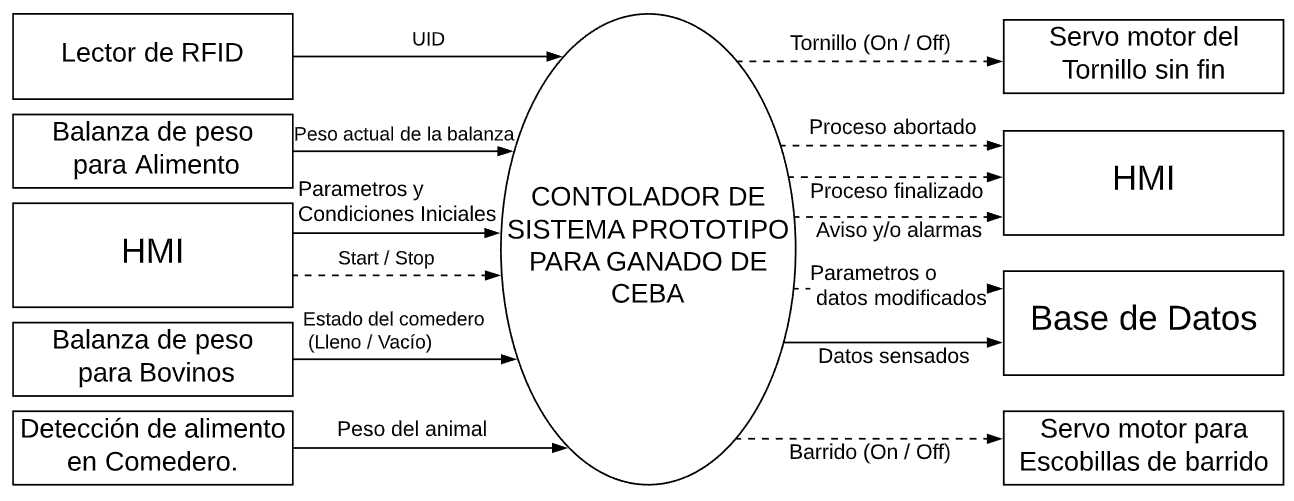
\includegraphics[scale=0.60]{img/contexto.png}
    \end{center}
    \caption{Diagrama de Contexto.}
    \label{contextopng}
\end{figure}

% \vspace{-45}
% \pagebreak

\subsubsection{Diagrama de estímulos}
Así como las máquinas y diagramas de estados son herramientas para comprender la evolución de los estados a partir de las entradas,
% Así Una manera simplificada para representar el comportamiento del sistema es mediante diagramas o maquinas de estados. De esta manera los cambios de estados o etapas pueden ser asimilados de manera simplificada y menos ambigua.
de forma similar, se puede representar la evolución lógica del sistema y sus entidades, mediante tablas de estímulos y transformaciones como la que se muestra a continuación:
\begin{table}[H]
    \centering
    \caption{Tabla de estímulos y transformaciones}
    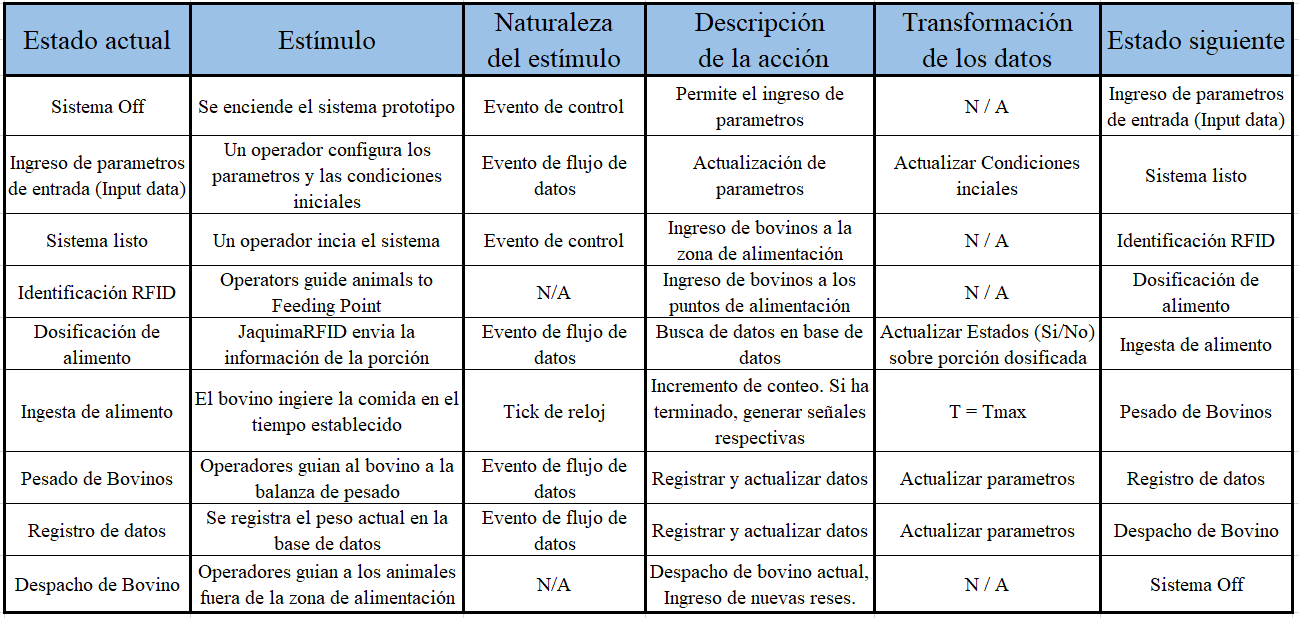
\includegraphics[scale=0.60]{img/estimulos.png}
\end{table}

%%% Tek

% \subsubsection{MSC}
% \subsubsection{SDL}

\subsubsection{Arquitectura}

Con el objetivo de simular un funcionamiento del sistema que evidencie situaciones cercanas a una implementación completa y real se considera un diseño lógico del comportamiento del sistema mediante la herramienta de software PragmaDev Studio. De esta forma se pueden organizar los procesos, canales de conexión y señales de comunicación entre los procesos.

Para este proyecto se diseña una arquitectura compuesta por un controlador, 11 procesos y un total de 33 señales de intercomunicación. Es importante aclarar que los procesos pueden ser usados por una misma entidad en diferentes cantidades que requieran del mismo proceso.

Esto quiere decir que para una implementación con 3 tolvas y 12 reses como se planteó en las consideraciones usadas para la Ecuación \ref{ecuaminima2} en la Sección \ref{subsissen}, no es necesario definir 12 procesos por cada RFID de cada bovino sino uno solo que aplique para las 12 reses. \\

\textbf{Los procesos \texttt{p[NombreProceso]} y los canales \texttt{c[NombreCanal]} pertenecientes a esta arquitectura son los siguientes:}
\begin{enumerate}
    % \begin{multicol}
    \item \texttt{pController}, como el proceso que representa al controlador.
    \item \texttt{pDatabase}, como el proceso que representa a la base de datos.
    \item \texttt{pRFIDsen}, en representación de los sensores lectores de RFID.
    \item \texttt{pBovineWSen}, en representación de la báscula de pesaje de bovinos.
    \item \texttt{pFoodWSen}, en representación de la báscula de pesaje de alimento.
    \item \texttt{pFoodPlateSen}, en representación de la detección de alimento en el comedero.
    \item \texttt{pFoodInTankSen}, en representación de la detección de alimento en la tolva.
    \item \texttt{pBrushHardware}, en representación del motor actuador de las escobillas de barrido fin.
    \item \texttt{pEndlessHardware}, en representación del motor actuador del tornillo sin.
    \item \texttt{pAlarmHardware}, en representación de las alarmas de interacción con el usuario.
    % \end{multicol}
% \end{enumerate}
% \pagebreak

% \textbf{Los canales de comunicación son los siguientes:}

% \begin{enumerate}
    % \begin{multicol}
    \item \texttt{cEnvCtrl}, Canal de comunicación entre el Controlador y el entorno
    \item \texttt{cCtrlRFID}, Canal de comunicación entre el Controlador y el lector RFID
    \item \texttt{cCtrlFoodWSen}, Canal de comunicación entre el Controlador y la báscula de pesaje de alimento
    \item \texttt{cCtrlPlate}, Canal de comunicación entre el Controlador y los sensores infrarrojos de detección de alimento en el comedero
    \item \texttt{cCtrlEnd}, Canal de comunicación entre el Controlador y el motor actuador del tornillo sin fin
    \item \texttt{cCtrlBase}, Canal de comunicación entre el Controlador y la base de datos
    \item \texttt{cCtrlBovineWSen}, Canal de comunicación entre el Controlador y la báscula de pesaje de bovinos
    \item \texttt{cCtrlTank}, Canal de comunicación entre el Controlador y la tolva
    \item \texttt{cCtrlBrush}, Canal de comunicación entre el Controlador y el motor actuador de las escobillas de barrido
    \item \texttt{cCtrlAlarm}, Canal de comunicación entre el Controlador y el actuador de la(s) alarma(s).
    % \end{multicol}
\end{enumerate}
\pagebreak


%\begin{figure}[H]
\begin{figure}
    \begin{center}
    	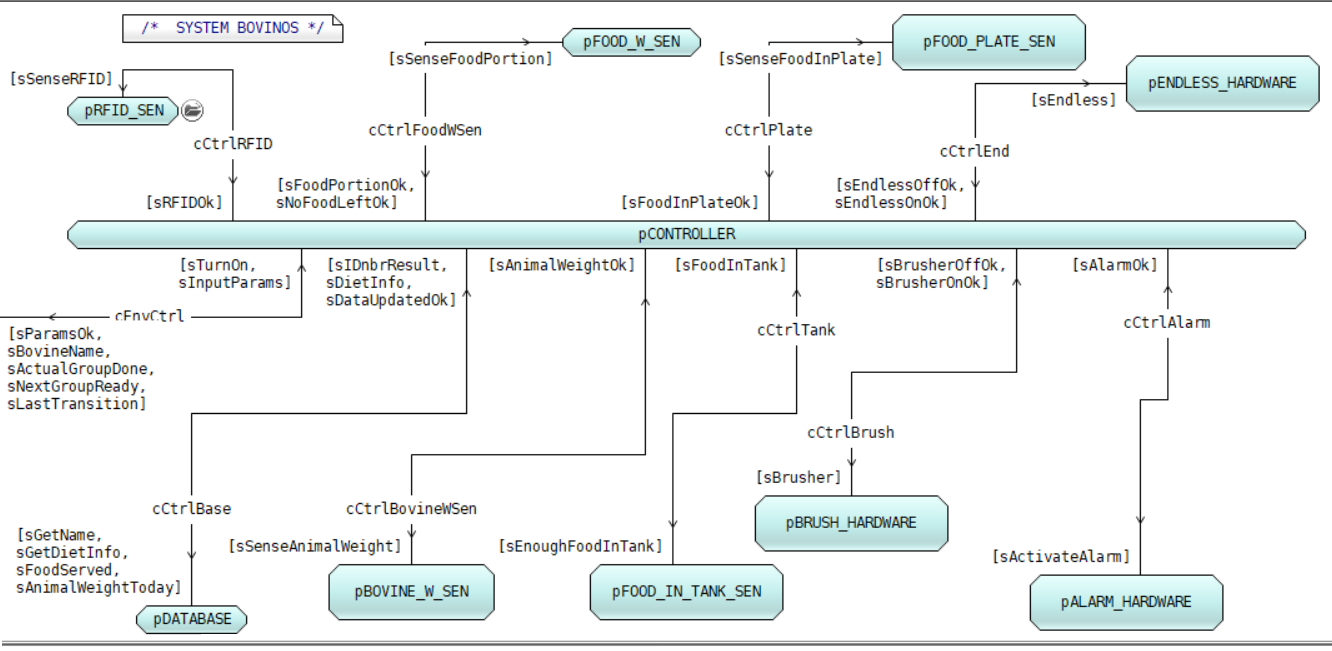
\includegraphics[scale=0.50,angle=90]{img/arqui.png}
    \end{center}
    \caption{Arquitectura, canales y señales de comunicación lógica del sistema prototipo.}
    \label{arquipng}
\end{figure}
%\pagebreak

\textbf{Las señales de interacción entre los procesos, el controlador y el entorno son las siguientes:}

\begin{figure}[H]
    \begin{center}
    	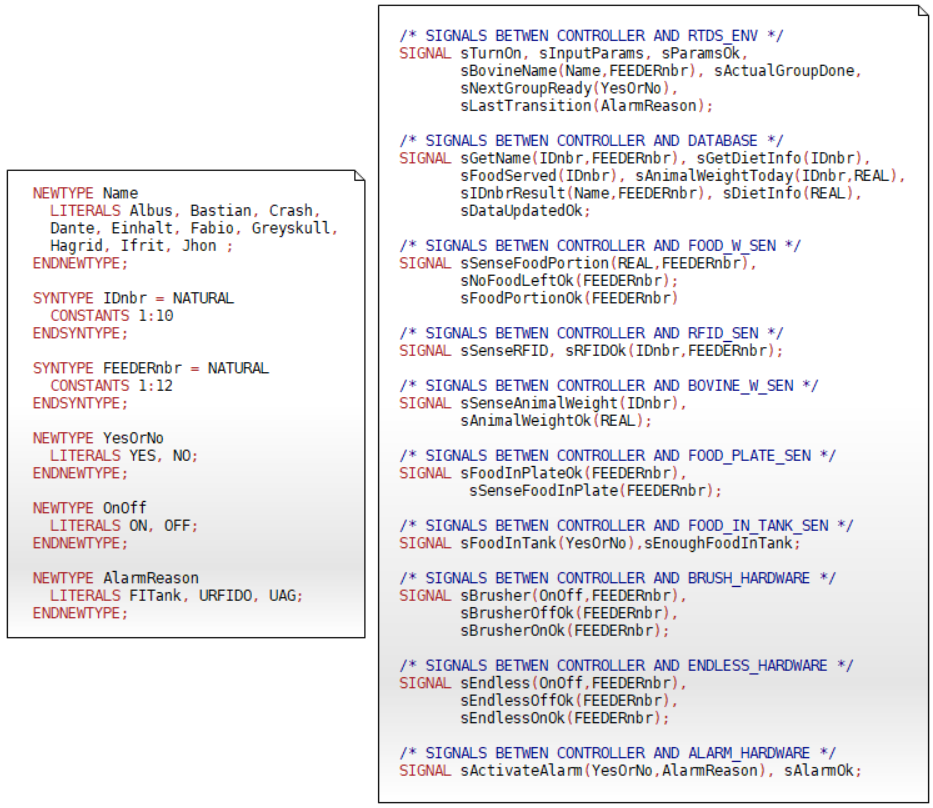
\includegraphics[scale=0.8]{img/senales2.png}
    \end{center}
    \caption{Tipos de señales de interacción entre los procesos, el controlador y el entorno}
    \label{senalespng}
\end{figure}

Con esto dicho, se procede a mostrar la arquitectura en la Figura \ref{arquipng}.

% \begin{itemize}
%     \item \textbf{Señales entre el Controlador y el Entorno}
%     \item \textbf{Señales entre el Controlador y la Base de datos}
%     \item \textbf{Señales entre el Controlador y la báscula de pesaje de alimento}
%     \item \textbf{Señales entre el Controlador y el lector RFID}
%     \item \textbf{Señales entre el Controlador y la báscula de pesaje de bovinos}
%     \item \textbf{Señales entre el Controlador y }
%     \item \textbf{Señales entre el Controlador y }
%     \item \textbf{Señales entre el Controlador y }
%     \item \textbf{Señales entre el Controlador y }
%     \item \textbf{Señales entre el Controlador y }
%     \item \textbf{Señales entre el Controlador y }
%     \item \textbf{Señales entre el Controlador y }
%     \item \textbf{Señales entre el Controlador y }
%     \item \textbf{Señales entre el Controlador y }
% \end{itemize}

%     \textbf{Bitácora del tiempo de PIPE 16/11/19:}
%     \textbf{xxx---   ----   ------   ---------   --------   -----xxx}
%     \textbf{xxx---   ----   ------   ---------   --------   -----xxx}
%     \textbf{Me falta:    Lo de la HMI \lonrightarrow{} PREGUNTAR A TAMURA.}
%     \textbf{xxx---   ----   ------   ---------   --------   -----xxx}
%     \textbf{xxx---   ----   ------   ---------   --------   -----xxx}

% \subsection{``Human-Machine Interface'' (HMI)}
% \subsubsection{Funciones}
% \subsubsection{FUNCIONES BASICAS (UNA A UNA)}
% \subsubsection{DISEÑO}

%
%
%establece el siguiente diagrama funcional del sistema (Ver Figura \ref{dfuncpng}):
%
%\begin{figure}[H]
%	\begin{center}
%		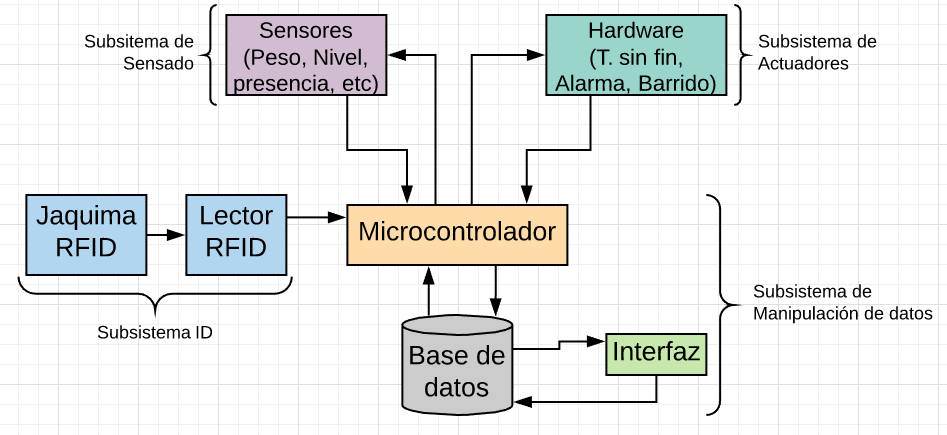
\includegraphics[scale=0.8]{img/dfunc.png}
%	\end{center}
%	\caption{Diagrama Funcional del sistema. \label{dfuncpng}}
%\end{figure}
%	 
